\documentclass[10pt,a4paper]{report}
\usepackage[utf8]{inputenc}
\usepackage[left=1in,right=1in,top=1in,bottom=1in]{geometry}
\usepackage{setspace}
\usepackage[british]{babel}
\usepackage[hidelinks]{hyperref}
\usepackage{array}
\usepackage{rotating}
\usepackage{natbib}
\usepackage{bibentry}
%\usepackage{chemfig}
%\usepackage[version=4]{mhchem}
\usepackage{siunitx}
\usepackage[table]{xcolor}
\usepackage{graphicx}
\usepackage{tabularx}
\usepackage{multirow}
\usepackage[font=small]{caption}
%\usepackage{newfloat}
%\usepackage{adjustbox}
%\usepackage{tocloft}
%\usepackage{cleveref}
\usepackage{bbkTitle}
\usepackage[outputdir=output/]{minted}
\usepackage{etoolbox}
\apptocmd{\sloppy}{\hbadness 10000\relax}{}{}

\newlength{\mytablewidth}

\onehalfspacing

% structure:
% 0. title
% 1. abstract
% 2. contents (chapters, sections, tables and figures)
% 3. introduction
% 4. materials and methods
% 5. results
% 6. discussion and conclusions
% 7. references

\begin{document}

\pagenumbering{arabic}
\supervisor{Dr. George Fitton}{SEAC Computational Scientist, Unilever}{george.fitton@unilever.com}
\supervisor{Dr. Alistair Middleton}{SEAC Computational Scientist Leader, Unilever}{alistair.middleton@unilever.com}
% \project{Master Thesis}
\author{Alberto Locca}
\title{Gene-to-gene Dynamic Methods for Time-Dependent Analysis for Biology Risk Assessments}

\maketitle

% 200-300 words
\begin{abstract}
Unilever's SEAC division is responsible for the safety and environmental impact assessment of Unilever products. To carry out this task in a sustainable and ethical manner, Unilever promotes the use of non-animal testing methods such as High Throughput Transcriptomics (HTTr) assays, which can be used to test the effect of different concentration of chemicals with different exposure time courses. Time can be factored in using different methodologies, but dynamic methods that model time as a continuous variable are not as well validated as other historically more established approaches.

This project focuses on developing a pipeline for the analysis of RNA-seq time series data by revising some of the most used and popular tools. In particular, the focus of this study is DPGP, a clustering tool that uses a Dirichlet process (DP) to determine the number of clusters, combined with a Gaussian process (GP) for modelling expression levels over time, and Bayesian inference to infer these parameters.

Using DPGP, this study was able (1) to reproduce very similar results to the ones published in its original paper, proving that DPGP can produce very consistent outputs, and (2) to assess its performance on simulated datasets with known characteristics and expected outcomes, which lead to inconclusive interpretations because of the assumptions used by the tool for generating those datasets.

Overall, DPGP has proven to be a potentially good addition to the pipeline. However, it needs to be investigated further in comparison to other similar tools and in the context of a real RNA-seq analysis pipeline.
\end{abstract}

\setcounter{page}{3}
\tableofcontents
\listoffigures
\listoftables

\chapter{Introduction}
\section{SEAC mission and project relevance}
Unilever's Safety and Environmental Assurance Centre (SEAC) division was founded in 1990 for assessing the safety and environmental impact of Unilever products. SEAC scientists work together with government scientists, regulators, and academics to carry out pioneering approaches that span different scientific fields -- \textit{i.e.} toxicology, microbiology, computational chemistry, bioinformatics, and mathematical modelling -- in order to ensure that Unilever products are safe for use and consumption as well as for the environment \citep{unileverLeadingSafetyEnvironmental2023}.

Unilever has a long history of promoting the use of non-animal testing methods for risk assessment, while trying to develop sustainable and viable alternatives, such as \textit{in vitro} assays and computational modelling \citep{unileverAlternativesAnimalTesting2023}. Besides the ethical discussion of which I will not enter into the merits, there is also scientific evidence to support the need for non-animal testing: many review studies reported that results from tests conducted in mouse, rat, and rabbit models are highly inconsistent in predicting toxic responses in humans \citep{vannormanLimitationsAnimalStudies2020}. Historically, there have been cases of drugs that were previously deemed safe during the clinical trial phases, and later had to be recalled for causing adverse effects, such as Vioxx from Merck which increases the risk of cardiovascular morbidity and mortality, and caused 38000 deaths and 88000 induced heart attacks \citep{juniRiskCardiovascularEvents2004}. Other notable cases include Thalidomide, which was withdrawn because it causes phocomelia and fetal deformations in pregnant women, despite there being no teratogenic effect reported in animal models, and Isuprel, which was originally developed for the treatment of asthma and caused an increase in deaths due to the high dosage approved in countries like the United Kingdom, Ireland, Australia and New Zealand \citep{jalbaThreeGenerationsOngoing2008}. Conversely, the opposite is also true: there are examples of safe drugs which are readily available that would have never passed toxicity testing if conducted in animal models, such as aspirin (that causes reproductive abnormalities and liver toxicity in rats), and paracetamol (that is toxic for cats and dogs) \citep{vannormanLimitationsAnimalStudies2020,villarIbuprofenAspirinAcetaminophen1998}.

Another reason in support of non-animal testing is the throughput: Unilever has a portfolio of more than \num{400} brands -- comprising food products, supplements, beauty and personal care products, beverages, and home care products -- therefore using animal models for testing all the compounds in all the formulations of all their products is simply not a viable option, both in terms of economical sustainability and in time and resource spending.
% need data
Animal testing is a very low throughput assay, and relatively expensive when compared to other \textit{in vitro} assays, which, by their nature, can more easily be automated, standardized, and scaled to ideally match the required characteristics for toxicity and risk assessment. An example is the \emph{Tox21} program, a consortium of public agencies, among whose main objectives are to develop better models for predicting the toxicity of an array of substances (the current goal is set to \num{10000}), and developing new \textit{in vitro} assays to reduce, refine, and replace the use of animal models \citep{lynchHighThroughputScreeningAdvance2023}. Among these technologies, in the current phase of the Tox21 program, the focus is on mid- to high-throughput gene expression screenings using human tissues and cells.

High Throughput Transcriptomics (HTTr) is a particular RNA sequencing (RNA-seq) technique designed to evaluate gene expression changes as effects of multiple conditions, such as treatment with different chemicals, increasing concentrations, or at different time points. In fact, time is an important factor that has often been overlooked in the past, but recent developments in transcriptome studies have allowed the design of more complicated experiments -- such as longitudinal studies -- in order to capture the biological processes in whole. For example, repeated exposure to small doses of a chemical compound (chronic dosage), or a spike dosage (acute phase) followed by a ``recovering'' phase. This is where this project begins: our main goal is to leverage the power of HTTr assays for toxicity and safety assessment by developing a new pipeline for the analysis of longitudinal data.

\section{Modelling longitudinal data}
RNA-seq can be used to evaluate transcriptional changes in genes already known (present in previous databases), but also to reconstruct the full RNA transcripts, even if they were not previously annotated. The sequencing process generates millions or billions of short sequences called \emph{reads} which are smaller portions of the original transcripts. The reads must then be matched to their original position inside the genome by aligning them to a reference. From this alignment, a final count is produced for each specific region of the genome, and a \emph{count matrix} is produced containing the number of reads per gene (or ``genome portion'') per different condition included in the experiment, which correspond to how much each gene is expressed \citep{frazeeDifferentialExpressionAnalysis2014,nagalakshmiTranscriptionalLandscapeYeast2008}. This is the starting point of many analytical pipelines.

For the scope of this project, the central principle is how time can be modelled and simultaneously account for expression variation over time. The ``common'' approach consists of the determination of differentially expressed genes (DEG) among different conditions. One of the most used tools is DESeq \citep{andersDifferentialExpressionAnalysis2010} and its later implementation DESeq2 \citep{loveModeratedEstimationFold2014a}, whose assumption is that each feature is independent, including time points, therefore time is modelled as a categorical variable. The software then performs linear regression for each feature (covariate) across all genes, and a fold change is calculated, indicating how much the expression level of a gene differs compared to the null model, which is when the expression level stays the same.

One obvious issue of this approach is that time cannot always be represented as a categorical variable, and by considering it as such one may oversimplify the biological system. This is an easy implementation of the already consolidated means for analysing genomic data that do not require existing models to be readapted or changed. This interpretation may work when we have less time points or when they are very distant, for example if we are studying a well-known biological mechanism for which we expect a certain outcome only after a certain amount of time has passed, but it poorly applies to an experiment where there are several repeated measurements of the same feature, and therefore each individual measure is no longer truly independent. 

To solve this issue, a possible different approach consists in treating time as a continuous variable, and modelling the gene expression using parametric statistics. One of the tools that uses this assumption is ImpulseDE2 \citep{fischerImpulseModelbasedDifferential2018}, which uses ``pulse functions'' to model gene expression levels over time by representing the transition between an initial state to a peak state, to a steady state. The goodness of fit is then evaluated by calculating a log-likelihood ratio test. One of the limitations of this approach is the limited number of the possible functions taken into account, which could recapitulate time-dependant gene expression. A more generalized method would be finding the function with the highest likelihood given the expression data, without specifying any function. This can be achieved by using Gaussian Processes (GPs), which are a type of non-parametric non-linear regression. Example tools that apply this concept are PairGP \citep{vantiniPairGPGaussianProcess2022} and GPrank \citep{topaGPrankPackageDetecting2018}.

\section{Choice of tool}
The choice of the tool examined in this study was based on review papers in the Literature -- two in particular -- detailing methods for RNA-seq data analysis. The first is a comparative study by \citet{spiesComparativeAnalysisDifferential2019}, in which the authors compare tools developed specifically for differential expression analysis of time course data, both on simulated and biological data.
The second is a review paper by \citet{ohTemporalDynamicMethods2021}, in which the authors describe a more comprehensive list of tools and dynamic strategies for studying non-periodical and periodical time course data, \textit{de facto} enriching the list of tools from \citeauthor{spiesComparativeAnalysisDifferential2019}.

From these two papers, a list of tools and their relative original papers was compiled, which was then used in a Python script to cross-search NCBI databases for resources linked to each article. Datasets linked to each publication entry were considered for two main reasons: the importance of reproducibility and the ability to test the consistency of those tools, therefore it is crucial that the authors made their data available, and having as many datasets available as possible for benchmarking the full RNA-seq analysis pipeline of this project. Lastly, the number of citation for each tool was captured in order to develop a ranking system (for a detailed description see section \ref{papers_metric}). The result is an updated table of which table \ref{tab:oh_metric} shows the most relevant columns.

This approach has three principal shortcomings:
\begin{enumerate}
    \item To perform cross-searches among NCBI databases, the NCBI E-Utilities software needs to be provided with the relative database ID (\textit{i.e.} PMID to search the Pubmed database). The list compiled from the review papers has DOI strings, which are extra fields in a Pubmed entry and can return unexpected results, like for the case of \emph{PairGP} (last row in table \ref{tab:oh_metric}): the Pubmed search returned 0 papers cited the PairGP paper, which could not be the case since it got cited at least once by \citeauthor{ohTemporalDynamicMethods2021}. This issue is due to a double DOI corresponding to the same article: one also present in the NCBI records, and one relative to the biorXiv pre-print, which is not accessible by simply using NCBI E-utilities.
    \item The average number of citations per year was used to rank the tools, which is not an objective metric for assessing the goodness of a paper, but it gives a rough estimate of the popularity it has among the scientific community. Generally speaking, a more popular tool would get included more often in analytical pipelines than a less popular one, which in turn would result in a more solid consensus. In fact, one of the challenges the computational community is facing is that there is still no consensus for the analysis of longitudinal RNA-seq data, which is also the reason why there is such a large number of tools available.
    \item Cross-searches among NCBI databases rely on the authors (or the publishers) to correctly list the resources linked to their publication. In this case, very few Pubmed entries also had the GEO Datasets accession linked, despite having it explicitly written in the text or in the supplementary material. Another possible reason for a GEO Datasets entry to not have an article linked to it could be if the data had been submitted well in advance of the publication, and it had not been updated.
\end{enumerate}

In spite of these problems, the script returned a reasonable outcome. It is worth noting that the tools for the analysis of periodical time courses are among the most popular. It may be because circadian rhythmic and cell-cycling changes have historically been more studied, or because some of these tools have been repurposed from older applications to also adapt to this type of analysis. Either way, since the HTTr assays used in this project involve non-periodical time course data, those tools are not taken into consideration. Within the non-periodical time course tools, the tools previously suggested by Unilever's external collaborators -- maSigpro and ImpulseDE2 -- are ranked among the highest positions. Lastly, some tools actually have publicly available datasets linked to their papers.

\section{DPGP}
This study focuses on the \emph{DPGP} (\emph{Dirichlet Process Gaussian Process}) tool based on the evaluation of the results of the NCBI cross-search from the previous section and shown in table \ref{tab:oh_metric}. Among the tools for the analysis of non-periodical time course, DPGP is one of the highest ranking, but unlike the others that were design to perform differential expression analysis, it has been developed for clustering time series of transcriptional data.

Clustering can be particularly useful in analysing RNA-seq data because it can be used to visualize the results, identify potential bias in the data (such as batch effects), but also to reduce the complexity by grouping genes into sub-categories of ``expression behaviours''. Furthermore, genes that belong to a cluster can be annotated ``by association'' assuming that they must share a common feature in order to be put in the same category, \textit{e.g.} regulatory pathway, molecular function, cellular location, sequence motif, etc. \citep{walkerPredictionGeneFunction1999}.

Unlike other clustering algorithms, DPGP does not need to pre-determine the number of clusters -- like in k-means clustering -- but it uses a \emph{Dirichlet process} (DP) to infer it from the data itself, combined with a Gaussian process (GP) for modelling expression levels over time.

\subsection{Bayesian inference}
DPGP uses both Dirichlet and Gaussian processes as priors, or in other words, the initial information about the data. Priors are used in Bayesian inference to infer the posterior distribution, which can be described as the updated initial information after factoring new observation (new knowledge) from the data.

In Bayesian inference, the posterior probability is calculated with Bayes' theorem, which uses the estimate of the probability of the hypothesis before factoring the data -- prior --, and the probability of observing the data given the parameters (or the model) -- likelihood -- to get the probability of observing the parameters given the data -- posterior.

Bayes' theorem general formula is:
\begin{displaymath}
    P(H|D) = \frac{P(D|H) \cdot P(H)}{P(D)}
\end{displaymath}
where
\begin{itemize}
    \item $H$ is the ``hypothesis'' event
    \item $D$ is the ``data'' or ``information'' event
    \item $P(H|D)$ is the posterior conditional probability (probability of observing the hypothesis given the data)
    \item $P(D|H)$ is the \emph{likelihood}, or prior conditional probability (probability of observing the data given the hypothesis)
    \item $P(H)$ is the prior, and
    \item $P(D)$ is the \emph{marginal likelihood}, or the probability of the observed data.
\end{itemize}

Lastly, to estimate the posterior distribution of the parameters of the mixed DPGP model, the software uses a Markov chain Monte Carlo method -- in particular, a Gibbs sampling algorithm -- to simultaneously infer the number of clusters \emph{and} the parameters that describe the gene expression trajectories for each cluster.

\subsection{Dirichlet process}
Dirichlet processes are often used in Bayesian models as a non-parametric prior because they allow not having to determine a certain parameter -- like in this case, the number of clusters -- but lets the data itself inform that decision.

The DP can be considered as a distribution over distributions, where the latter can be parametrized as the ``mean'' of the DP, with a ``concentration'' parameter that determines how closely the sampled distributions are to the base ``mean'' distribution.

DP can be used for clustering because distributions sampled from a DP can be considered an isolated group (or cluster) from which the data comes from.

\begin{figure}[!ht]
    \centering
    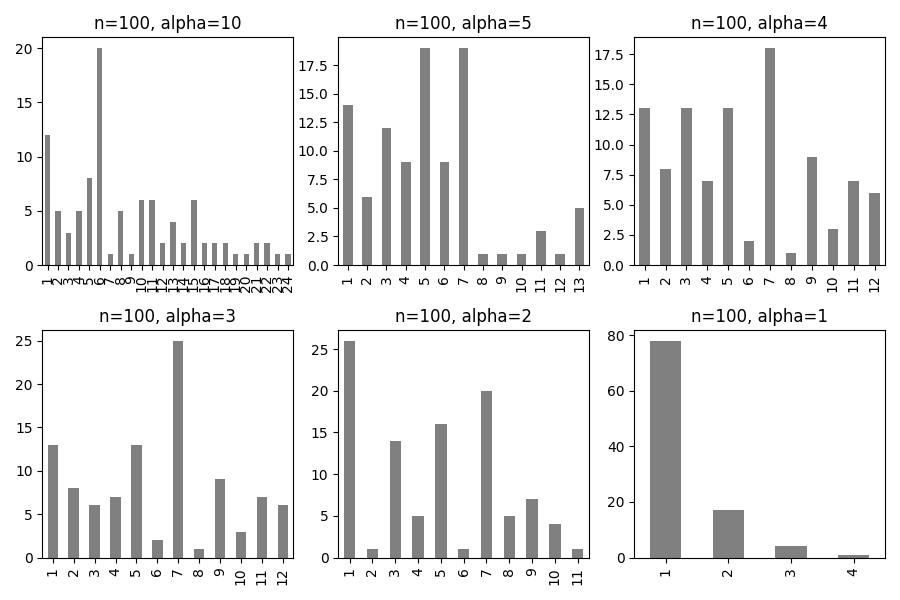
\includegraphics[width=.9\textwidth]{src/chinese_restaurant.png}
    \caption[Chinese restaurant process example]{Chinese restaurant process example. The picture shows the effect of the concentration parameter $\alpha$, which affects the probability of creating a new group -- or table, or cluster -- with a fix number to be organized. Each bar represents the number of assigned values to that group. As the $\alpha$ value decreases, also the number of groups gets lower, with a maximum of 24 groups for $\alpha=10$, and a minimum of 4 for $\alpha=1$. The default value used in the DPGP software is $\alpha=1$.}\label{intro:crp}
\end{figure}

A classical example used to visualize DP is the Chinese restaurant process (CRP). In this metaphor, people enter an imaginary Chinese restaurant, and they have two choices: sit to a table where there are other people sitting there, or sit to a new empty table. The probability for the first choice is proportional to the number of people already at the table, meaning it's more likely to sit at a table with many people than few. The probability for the second choice is proportional to the concentration parameter. The script \texttt{dp\_chinese\_restaurant.py} recreates this simple example, and produces figure \ref{intro:crp}, which shows the effect of the concentration parameter: the lower the value, the more ``concentrated'' people are, meaning it is harder for people to sit to new tables.

At the end of the CRP, the result is a particular probability distribution of assignments, which is one of the possible distributions that could be sampled from the DP.

\subsection{Gaussian process}
DPGP uses Gaussian process (GP) as a prior for each specific cluster over the range of possible gene expression trajectories over time.

In this case, the base distribution from the DP captures the distribution of all the parameters for each cluster-specific GP, which in turn captures all the functions that model the data points (gene expression over time).

GP also depends on other parameters, expressed as the hyperprior distribution Inverse Gamma, which can be parametrized as $\alpha$ and $\beta$ variables that capture respectively the shape and rate of the Inverse Gamma distribution. In the DPGP software these two parameters are set to $\alpha=12$ and $\beta=2$ based on the authors experience, but they can be altered to allow for different degree of variability in the data; in particular, lowering the shape parameter will allow for a greater marginal variance within each cluster.


\chapter{Materials and Methods}
\section{Papers metric for tool selection}\label{papers_metric}
Starting from the review paper by \citeauthor{ohTemporalDynamicMethods2021}, in which the authors describe a list of available tools and dynamic strategies for studying non-periodical and periodical time course data, table \ref{tab:oh} was compiled by collecting all the tools discussed by \citeauthor{ohTemporalDynamicMethods2021}. The ones for handling batch effect have not been included (which are listed in Table 3 of the original paper; see \emph{Original table} column in table \ref{tab:oh}) because batch effects are not taken into account for the scope of the pipeline of this project, but they may be included in future implementations.

\begin{table}[!ht]
    \centering\footnotesize
    \begin{tabular}{lllll}
\textbf{Name} & \textbf{Original table} & \textbf{Type} & \textbf{Time course} & \textbf{DOI} \\
Next maSigpro & Table 1 & Dynamic gene-by-gene & Non-periodical & 10.1093/bioinformatics/btu333 \\
DyNB & Table 1 & Dynamic gene-by-gene & Non-periodical & 10.1093/bioinformatics/btu274 \\
EBSeq-HMM & Table 1 & Dynamic gene-by-gene & Non-periodical & 10.1093/bioinformatics/btv193 \\
Ngsp & Table 1 & Dynamic gene-by-gene & Non-periodical & 10.1093/bioinformatics/btu699 \\
Lmms & Table 1 & Dynamic gene-by-gene & Non-periodical & 10.1371/journal.pone.0134540 \\
timeSeq & Table 1 & Dynamic gene-by-gene & Non-periodical & 10.1186/s12859-016-1180-9 \\
splineTimeR & Table 1 & Dynamic gene-by-gene & Non-periodical & 10.1371/journal.pone.0160791 \\
ImpluseDE2 & Table 1 & Dynamic gene-by-gene & Non-periodical & 10.1093/nar/gky675 \\
Trendy & Table 1 & Dynamic gene-by-gene & Non-periodical & 10.1186/s12859-018-2405-x \\
AR & Table 1 & Dynamic gene-by-gene & Non-periodical & 10.1038/s41598-018-37397-7 \\
MAPTest & Table 1 & Dynamic gene-by-gene & Non-periodical & 10.1111/biom.13144 \\
TimeMeter & Table 1 & Dynamic gene-by-gene & Non-periodical & 10.1093/nar/gkaa142 \\
PairGP & Table 1 & Dynamic gene-by-gene & Non-periodical & 10.1016/j.compbiomed.2022.105268 \\
GPrank & Table 1 & Dynamic gene-by-gene & Non-periodical & 10.1186/s12859-018-2370-4 \\
Dream & Table 1 & Dynamic gene-by-gene & Non-periodical & 10.1093/bioinformatics/btaa687 \\
rmRNAseq & Table 1 & Dynamic gene-by-gene & Non-periodical & 10.1093/bioinformatics/btaa525 \\
JTK\_CYCLE & Table 2 & Dynamic gene-by-gene & Periodical & 10.1177/0748730410379711 \\
MetaCycle & Table 2 & Dynamic gene-by-gene & Periodical & 10.1093/bioinformatics/btw405 \\
RAIN & Table 2 & Dynamic gene-by-gene & Periodical & 10.1177/0748730414553029 \\
DODR & Table 2 & Dynamic gene-by-gene & Periodical & 10.1093/bioinformatics/btw309 \\
LimoRhyde & Table 2 & Dynamic gene-by-gene & Periodical & 10.1177/0748730418813785 \\
Tcgsaseq & Table 4 & Coherent gene-to-gene & Non-periodical & 10.1093/biostatistics/kxx005 \\
FunPat & Table 4 & Coherent gene-to-gene & Non-periodical & 10.1186/1471-2164-16-S6-S2 \\
DPGP & Table 4 & Coherent gene-to-gene & Non-periodical & 10.1371/journal.pcbi.1005896 \\
LPWC & Table 4 & Coherent gene-to-gene & Non-periodical & 10.1186/s12859-019-3324-1 \\
\end{tabular}

    \caption[Collection of tools as listed in the paper by \Citeauthor{ohTemporalDynamicMethods2021}]{Collection of tools as listed in the paper by \citet{ohTemporalDynamicMethods2021}. \emph{Type} and \emph{Time course} are two of the labels used to classify the different tools. For convenience, a \emph{DOI} column was included for easy searching.}
    \label{tab:oh}
\end{table}

A Python program was then used to select the most relevant tools among the listed ones by accomplishing two major tasks:
\begin{enumerate}
    \item searching for databases linked to the publication,
    \item developing a metric on which papers could be scored.
\end{enumerate}

The script is a basic wrapper for the NCBI E-utilities \citep{bethesdaEntrezProgrammingUtilities2010} Python implementation within the \texttt{Biopython} module \citep{cockBiopythonFreelyAvailable2009}. For each tool, the listed publication DOI string was used to search the NCBI databases for resources linked to each paper, in the attempt to assess if the datasets used in the publications were made available in public databases, namely NCBI GEO Datasets -- a curated repository of gene expression data -- and NCBI BioProject -- a collection of biological data per project/effort (meaning each entry contains descriptive information about the experimental data, and could link to multiple resources and datasets).
In order to score the tools, the number of citation for each paper was used to get the average number of citations per year by calculating the difference in days between the current date and the date of publication, and dividing it by the number of days in a year (365.25, accounting for leap years). Note that because of this, every future execution will produce different values. The result is an updated version of the previous table \ref{tab:oh} with six extra columns: PMID (Pubmed ID), publication date (formatted as year-month-day), number of citations, average number of citations per year, GEO Datasets ID, and BioProject ID. Table \ref{tab:oh_metric} shows a shorter version (for readability purpose) of the script output.

\begin{table}[!ht]
    \centering\footnotesize
    \begin{tabular}{llc>{\centering}m{2.3cm}cc}
\textbf{Name} & \textbf{Time course} & \textbf{Cited by} & \textbf{Average yearly citations} & \textbf{GEO Dataset ID} & \textbf{Bioproject ID} \\
JTK\_CYCLE & Periodical & 482 & 37.50 &  &  \\
MetaCycle & Periodical & 212 & 28.47 &  &  \\
RAIN & Periodical & 148 & 16.81 &  &  \\
Next maSigpro & Non-periodical & 143 & 15.59 &  &  \\
Dream & Non-periodical & 52 & 14.60 &  &  \\
ImpluseDE2 & Non-periodical & 53 & 8.79 &  &  \\
DPGP & Non-periodical & 54 & 8.62 & 200104714 & 413586 \\
DODR & Periodical & 46 & 6.17 &  &  \\
LimoRhyde & Periodical & 26 & 5.54 &  &  \\
EBSeq-HMM & Non-periodical & 44 & 4.99 &  &  \\
DyNB & Non-periodical & 33 & 3.61 &  &  \\
Trendy & Non-periodical & 16 & 3.24 &  &  \\
splineTimeR & Non-periodical & 20 & 2.75 &  &  \\
Lmms & Non-periodical & 20 & 2.37 &  &  \\
Ngsp & Non-periodical & 18 & 2.05 &  &  \\
FunPat & Non-periodical & 16 & 1.96 &  &  \\
rmRNAseq & Non-periodical & 8 & 1.95 &  &  \\
timeSeq & Non-periodical & 11 & 1.48 &  &  \\
LPWC & Non-periodical & 6 & 1.36 &  &  \\
Tcgsaseq & Non-periodical & 7 & 0.99 &  &  \\
GPrank & Non-periodical & 4 & 0.78 &  &  \\
AR & Non-periodical & 4 & 0.74 &  &  \\
TimeMeter & Non-periodical & 1 & 0.29 & 200130438 & 540258 \\
MAPTest & Non-periodical & 1 & 0.21 &  &  \\
PairGP & Non-periodical & 0 & 0.00 & 200154467 & 646394 \\
\end{tabular}

    \caption[Paper metrics table obtained from table \ref{tab:oh}]{Paper metrics table obtained from table \ref{tab:oh} after running the script \texttt{entrez.py} (see \ref{code}). Tools are listed in descending order by \emph{Average yearly citations}. Some columns have been omitted for readability.}
    \label{tab:oh_metric}
\end{table}

\section{DPGP setup}
The DPGP software is available as a Python program at the GitHub repository \url{https://github.com/PrincetonUniversity/DP_GP_cluster} (last updated 22 September 2017). Since its publication \citep{mcdowellClusteringGeneExpression2018}, it has not been updated, and it looks like it is not actively maintained.

In the repository, it states that it has been tested on GNU/Linux systems with Python 2.7 and Anaconda distributions, so to mirror the installation steps suggested by the authors, a conda environment was created with that specified Python version together with the version of the required packages on which DPGP depends -- \textit{i.e.} \texttt{scikit-learn}, \texttt{pandas}, \texttt{GPy}, \texttt{numpy}, \texttt{scipy}, \texttt{matplotlib}, and \texttt{cython}. The environment file was exported with all packages dependencies and made it available in the code repository (see \ref{code}), both in text and YAML format for convenience.

Next, after activating the environment, DPGP is installed from its official GitHub repository using \texttt{pip}. To recreate the installation process, run the following commands:
\begin{minted}{bash}
conda create --name dpgp --file DPGP_conda_env.txt
conda activate dpgp
pip install git+https://github.com/PrincetonUniversity/DP_GP_cluster.git
conda deactivate
\end{minted}

\section{Response to \texorpdfstring{H\textsubscript{2}O\textsubscript{2}}{H2O2} in archaebacterium \textit{Halobacterium salinarum}}
As test case, \citeauthor{mcdowellClusteringGeneExpression2018} used a real biological dataset previously published by their own group \citep{sharmaRosRTranscriptionFactor2012}, which can be downloaded at the \href{https://www.ncbi.nlm.nih.gov/geo/query/acc.cgi?acc=GSE33980}{GEO accession GSE33980}. In that original work, the authors studied the transcriptional response of the archaebacterium \textit{Halobacterium salinarum} to the treatment with hydrogen peroxide. 

The choice of using this dataset was backed by the fact that the original study was conducted in a relatively simple system with a small genome, and the results had a clear biological meaning in response to a single stimulus over time. 

\subsection{Original experimental design}\label{biodata}
\textit{Halobacterium salinarum} strains were cultured under standard conditions (\SI{37}{\degreeCelsius} for 48 hours under continuous shaking) until the growth rate reached a mid-logarithmic phase. For RNA extraction, \SI{4}{\milli\litre} culture aliquots were removed prior to the addition of \SI{25}{\milli\mole} H\textsubscript{2}O\textsubscript{2}, and at five time points following H\textsubscript{2}O\textsubscript{2} addition -- at 10, 20, 40, 60, and 80 minutes. Each measurement had two technical replicates, accounting for 12 total measurements per strain -- a control strain, termed \emph{ura3}, and a mutant strain, termed either \emph{d258} or \emph{$\Delta$rosR}. The mutant strain has a deletion that results in the absence of the transcription factor rosR, which is found to have a protective effect to oxidative stress, such as the exposure to H\textsubscript{2}O\textsubscript{2}.

Gene expression was evaluated using Agilent microarray systems -- \href{https://www.ncbi.nlm.nih.gov/geo/query/acc.cgi?acc=GPL14876}{GEO platform accession GPL14876} -- which contains 2410 non-redundant open reading frames of the \textit{H. salinarum} NRC-1 genome. Raw data were analysed using R Bioconductor \texttt{m-array} \citep{paquetMarrayExploratoryAnalysis2023} and \texttt{limma} packages \citep{ritchieLimmaPowersDifferential2015,smythLimmaLinearModels2023}: background was subtracted using \texttt{normexp}, Loess normalization was performed within each array, and quantile normalization between all arrays. Any probe for each gene lying outside the 99\textsuperscript{th}\% confidence interval was removed using Dixon's test. The remaining probe intensities for each gene were averaged and log2 ratios were calculated, yielding one expression ratio per gene. This processed count table was made available in the GEO Dataset entry supplementary files as \texttt{GSE33980\_average\_data.txt.gz}.

\citeauthor{sharmaRosRTranscriptionFactor2012} then used the Gaggle data analysis web environment \citep{shannonGaggleOpensourceSoftware2006} to perform statistical analysis and differential expression analysis of the data. They identified 626 DEGs which they clustered using a k-means algorithm.

\subsection{Data processing and clustering}\label{preprocess}
In order to mirror the analysis conducted by \citeauthor{mcdowellClusteringGeneExpression2018}, a series of Python scripts were used to perform the following steps.
\paragraph{Data collection} A python script -- \texttt{geo\_DPGP.py} -- that uses the GEOparse package \citep{gumiennyGEOparsePythonLibrary2021} to access each GEO Dataset entry provided -- in this case \href{https://www.ncbi.nlm.nih.gov/geo/query/acc.cgi?acc=GSE33980}{GEO accession GSE33980} -- and download all the supplementary data listed -- in this case the processed count table \texttt{GSE33980\_average\_data.txt.gz}. A second Python script -- \texttt{gse33980\_suppl.py} -- that extrapolates the list of the names of all 626 DEGs, which was included in an Excel table in the supplementary materials of the paper by \citeauthor{sharmaRosRTranscriptionFactor2012}.
\paragraph{Data pre-processing} In order to run DPGP, the data have to be formatted in a specific way: each condition -- control and mutant strains -- has to be run separately, and the count table has to be a tab formatted table where the first column contains the gene identifiers (or any other type of label), and the column names must represent each time point. Each replicate has to be separated in its own count table, but they have to be input together to DPGP.

The Python script \texttt{gse33980\_data\_preprocess.py} was written for this purpose. It filters the dataset obtained in the previous step for only the 626 DEGs (which were actually 616), and generates a ``metadata'' table from the measurement labels to ulteriorly subset the data into the desired format: retains only the measurements for the group treated with H\textsubscript{2}O\textsubscript{2}, splits the dataset into the two strains, which it ulteriorly splits into single replicates.

DPGP takes as inputs the list of all the expression count tables replicates, but they must have matching number of time points. In this case, the second replicate of the mutant strain is missing the \SI{20}{\min} time point, which is present in all other conditions. DPGP was run using different inputs combination -- excluding that time point in the mutant group only, or in both groups (data not shown) -- but the results that more closely match the ones from \citeauthor{mcdowellClusteringGeneExpression2018} are obtained by filling the missing measurements using the data from the first replicate. When both strains were treated in this way -- using the same \SI{20}{\min} time point of the first replicate in both tables -- the results were again discordant from the ones obtained in the DPGP paper (data not shown).

\paragraph{Clustering} Finally, a bash script -- \texttt{dpgp\_gse33980\_paper.sh} -- executes DPGP and performs the clustering, using the same flags that corresponds to the parameters used in the paper: \texttt{--fast} will run DPGP in ``fast'' mode, which \citeauthor{mcdowellClusteringGeneExpression2018} used throughout their paper. \texttt{--sigma\_n2\_shape} and \texttt{--sigma\_n2\_rate} are the hyperparameters $\alpha$ and $\beta$ respectively, that can be varied to allow for greater variability by reducing the shape parameter. In the paper, they stated that they used $\alpha=6$ (default 12) and $\beta=2$ (default 2), because these are microarray data. Finally, \texttt{--plot} will output cluster images like the ones shown in the original work (see figure \ref{img:paper}), in the format specified by \texttt{-p}.

\subsection{Results comparison}
\citeauthor{mcdowellClusteringGeneExpression2018} clustered gene trajectories for each of the control and mutant strains in independent DPGP modelling runs, so to compare them and determine the gene cluster assignment changes in response to the mutation, they computed the Pearson correlation coefficient on all the mean trajectories combinations of clusters. The clusters with the highest coefficients were considered equivalent across the two strains. To test the significance of gene switching between equivalent clusters, the authors used the Fisher's exact test.

In order to reproduce this analysis, the Python script \texttt{gse33980\_dpgp\_results.py} first calculates the mean expression trajectories of each cluster using the posterior cluster model. This script has been adapted from function present in the DPGP code, \texttt{plot.py} in particular. The script also produces single plots for each cluster (used in the section \ref{eq_clust}), instead of the standard graphical output of DPGP, \label{standard_output} which has six cluster plots per image, and alternative similarity matrix images for both strains (without the default dendrogram, see figure \ref{img:heatmap}), and with the gene order rearranged for the mutant strain (see figure \ref{img:heatmap_alt}) to mirror the image shown in figure \ref{img:paper} panel N. Since this script rely on the DPGP Python module, it must be run in the conda environment with the following command:
\begin{minted}{bash}
conda run -n dpgp python DPGP/src/gse33980_dpgp_results.py
\end{minted}

A second Python script was written -- \texttt{gse33980\_dpgp\_analysis.py} -- to calculate the Pearson correlation coefficient -- using the \texttt{pearsonr} function of the Python \texttt{SciPy} module \citep{virtanenSciPyFundamentalAlgorithms2020} -- of all the possible pairs of posterior cluster mean expression trajectories, and determine which are the equivalent clusters by selecting the pair with the highest value of $r$. The matrix of $r$ values of the full pairwise comparisons is shown in table \ref{tab:pearson}. The full 3D matrix of $r$ and $p$ values is saved as a \texttt{numpy} binary file -- \texttt{geo\_correlation\_matrix.npy}.

The same script also extrapolates from the DPGP results (specifically from the optimal clustering output, which is a table containing the list of all genes and their corresponding cluster label) the number of co-clustered genes in each possible pairwise combination of control \textit{vs.} mutant clusters, and produces table \ref{tab:cocluster}, where the highlighted cells correspond to the number of genes that are clustered in the equivalent cluster, meaning that they maintain the same expression behaviour over time.
Table \ref{tab:cocluster} is used to calculate the contingency tables of the equivalent cluster pairs, which in turn are used to calculate the Fisher's exact test.
Each contingency table has the following format:

\begin{center}
\begin{tabular}{>{\bfseries\centering}m{3.5cm} | >{\centering}m{3.5cm} | >{\centering}m{3.5cm} p{0pt}}
 & \textbf{Belong to mutant cluster \textit{n}} & \textbf{Do NOT belong to mutant cluster \textit{n}} & \\ \hline
Belong to control cluster \textit{m} & $x$ & $y=row - x$ & \\ \hline
Do NOT belong to control cluster \textit{m} & $z=col - x$ & $616 - (x+y+z)$ & \\
\end{tabular}
\end{center}

Where
\begin{itemize}
    \item $x$ is the number of genes belonging to both clusters
    \item $y$ is the number of remaining genes in the control cluster
    \item $z$ is the number of remaining genes in the mutant cluster
    \item the last cell is the number of genes not belonging to any of those two clusters, which correspond to the total number of genes -- \num{616} in this case -- minus the genes in either one of the two clusters $m$ and $n$ 
\end{itemize}

Finally, a summary of the statistical analysis of the equivalent cluster pairs is produced (see table \ref{tab:eq_clust}), showing for each control cluster which is the equivalent mutant cluster, the Pearson correlation $r$ and $p$ values, and Odds ratio and Fisher's exact test (FET) $p$ value, which are calculated using the \texttt{fisher\_exact} function within the same \texttt{SciPy} module \citep{virtanenSciPyFundamentalAlgorithms2020}. The last column contains the number of genes that show a different gene expression dynamic (also expressed as a percentage of the total number of genes of control cluster), which was calculated from the relative contingency table.

\section{Data simulation}
Since the pipeline this project is building will perform differential expression analysis using, among other tools, \texttt{ImpulseDE2} \citep{fischerImpulseModelbasedDifferential2018}, DPGP was also tested in this study on toy datasets that have gone through the pipeline. 
\subsection{Datasets generation}\label{simulation}
\paragraph{ImpulseDE2 installation} ImpulseDE2 is available as an R package at the GitHub repository (\url{https://github.com/YosefLab/ImpulseDE2}, last updated 14 September 2022), and in Bioconductor version 3.10 (\url{https://bioconductor.org/packages/3.10/bioc/html/ImpulseDE2.html}, version 1.10.0). The package has been removed starting from Bioconductor version 3.13.
For this reason, ImpulseDE2 has been downloaded from the GitHub repository and included in an R project (available in the repository of this study, see section \ref{code}) using \texttt{renv}, which creates a \texttt{lockfile} containing the information of all the packages used. To recreate the installation process, open the R project \texttt{impulseDE2.Rproj}, and run the following command in an R console:
\begin{minted}{R}
renv::restore()
\end{minted}

\paragraph{Dataset creation and DE analysis} The following steps were recreated from the tutorial present in the \texttt{ImpulseDE2} vignette. In order to produce the simulated datasets to use in this study, the \texttt{simulateDataSetImpulseDE2} function was used, which can generate a specified amount of gene expression vectors modelled according to four possible functions:
\begin{enumerate}
    \item \emph{constant}, which produces constant gene count with no effect over time,
    \item \emph{impulse}, where the effect over time is represented from an initial state that shifts to a ``peak'' state, and to a ``steady'' state,
    \item \emph{linear}, where the gene counts follow a linear trajectory over time, and
    \item \emph{sigmoid}, which produces genes counts with a sigmoidal time progression.
\end{enumerate}

Two datasets were created: one with \num{400} genes using the linear function only (\emph{linear dataset}), and a second one using the constant, impulse, and linear functions with \num{200} genes each, for a total of \num{600} genes (\emph{mixed dataset}). Both datasets have 8 time points and three replicates. These numbers were chosen to have a starting size comparable to the one from the real biological dataset (which has 626 genes, see section \ref{biodata}), and still be relative fast to cluster with DPGP.

DE analysis was performed with the \texttt{runImpulseDE2} function, which in this case -- where no alternative condition has been provided -- compares gene expression levels against a constant expression model with no variations over time. The resulting list of DEG was used in the next step to filter the whole dataset before running DPGP.

\subsection{Clustering and analysis}
Next, a processing step was performed, similar to the one described in section \ref{preprocess}, which is necessary for running DPGP.
\paragraph{Data pre-processing}
The Python script \texttt{simulated\_data\_preprocess.py} reads each of the two datasets -- linear and mixed -- and produces the individual expression matrices for each replicate, which are then provided together as the input of DPGP. For each dataset, the script also creates two alternative sub-datasets: one with the full list of genes, and a second one with only DEGs, for a total of four datasets.

\paragraph{Clustering}
DPGP was run on each one of these sub-datasets -- with the full list of genes, or only DEGs, from each simulated dataset, linear or mixed -- using the bash script \texttt{dpgp\_simulated.sh}. The parameters used are again similar to the ones used on the biological data: \texttt{--fast} is used to run DPGP in ``fast'' mode, and \texttt{--plot} to produce the standard graphical output in the format specified by \texttt{-p}. The script also iteratively pass a value for the $\alpha$ hyperparameter (\texttt{--sigma\_n2\_shape}), which is used to allow for variability within the data. Not knowing how variable these datasets are (since the \texttt{simulateDataSetImpulseDE2} function also includes dispersion factors), an array of values was chosen: $\alpha=12$ (the default), $9$, $6$ (the value used by \citeauthor{mcdowellClusteringGeneExpression2018}), and $3$.

\paragraph{Result analysis}
The results of each DPGP run are then reformatted using the Python script \texttt{simu\-lated\_dpgp\_results.py}, which produces the images shown in section \ref{res:simulated}, with similar quality to the one described in section \ref{standard_output}. Since this script rely on the DPGP Python module, it must be run in the conda environment with the following command:
\begin{minted}{bash}
conda run -n dpgp python DPGP/src/simulated_dpgp_results.py      
\end{minted}

Lastly, the Python script \texttt{simulated\_dpgp\_analysis.py} evaluates DPGP ability to capture groups of genes generated by different \texttt{ImpulseDE2} model functions. The script takes advantage of the fact that the genes are in sequential order in the generated dataset, where the first are the number of constant genes, followed by the one generated by the impulse function, then the linear, and finally the sigmoid. The script takes all the DPGP results from the mixed sub-datasets and produces summary tables showing the count of genes per cluster that were generated by the three different functions -- constant, impulse, and linear. The background gradient is the result of a row-wise comparison: the darker the colour, the higher number of genes generated from that function belong to a specific cluster.

\section{Code availability}\label{code}
All the code used in this dissertation is available at the GitHub repository \url{https://github.com/bio-tilion/AL_MScProject.git}.


\chapter{Results}
This study was conducted to test the viability of the DPGP tool on longitudinal RNA-seq data, with the end goal of including it in the project pipeline whether it produces reasonably sound results. For this purpose, DPGP was first used to recreate the findings published in its original paper \citep{mcdowellClusteringGeneExpression2018}, and then tested it on simulated datasets, as a way to assess its behaviour in a controlled setting environment with known expectations.

\section{Reproducing DPGP results}\label{res:geo}
The objective of this study was to obtain a result that is as close as possible to the analysis done by \citeauthor{mcdowellClusteringGeneExpression2018} in the DPGP paper, by focusing on the dataset obtained from the treatment of \textit{Halobacterium salinarum} with H\textsubscript{2}O\textsubscript{2}. Figure \ref{img:paper} -- which is labelled \emph{Fig 2} in the original paper -- shows the plots that were recreated in this study.

\begin{figure}[!ht]
    \centering
    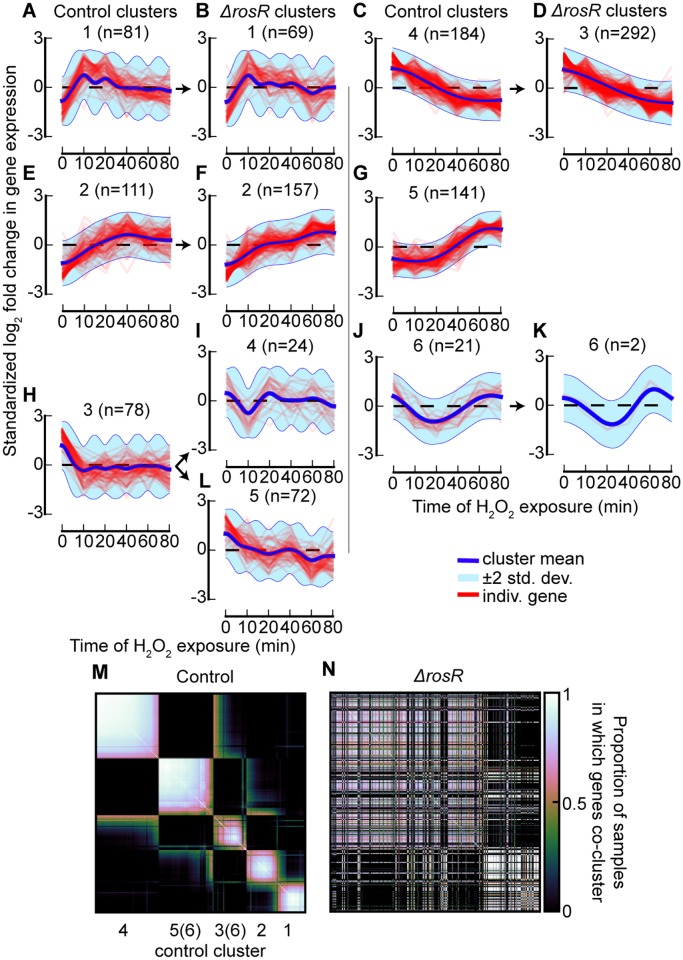
\includegraphics[width=.65\textwidth]{../DPGP/papers/pcbi.1005896.g002.jpg}
    \caption[Oxidative stress response clusters from \citeauthor{mcdowellClusteringGeneExpression2018}]{Original figure of the oxidative stress response clusters from \citealp{mcdowellClusteringGeneExpression2018}. (A-L) Gene expression trajectories for each cluster. Red lines are standardized $\log_{2}$ fold change of single gene expression. Blue lines are the posterior cluster mean expression levels. The first and third columns (panels A, E, H, C, G, and J) show control clusters, and the second and fourth columns (panels B, F, I, L, D, and K) the mutant clusters. The arrows point at the equivalent mutant cluster based on the Pearson correlation coefficient of the mean trajectories. (M, N) Heatmaps showing the proportion of sampled genes that cluster with every other gene for the control strain (M), and for the mutant $\Delta$rosR strain (N). The gene order has been determined by Ward's linkage for the control, and for the mutant it has been assigned the same order as the control.}\label{img:paper}
\end{figure}

First, the \href{https://www.ncbi.nlm.nih.gov/geo/query/acc.cgi?acc=GSE33980}{GEO GSE33980 dataset} was downloaded, which also contains data from a second experiment where \textit{H. salinarum} has been treated with a different compound. The pre-processing step filters that data out and prepares the expression matrices to input into DPGP (for the full description, see \ref{preprocess}). In the original work that produced the GEO dataset \citep{sharmaRosRTranscriptionFactor2012}, the authors identified 616 differentially expressed genes (DEGs) which they clustered using a k-means algorithm. \citeauthor{mcdowellClusteringGeneExpression2018} ran DPGP only on the DEGs and not the whole dataset, but it was not shared among the supplementary material of the DPGP paper, so the list of DEGs was retrieved from the supplementary material of the paper by \citeauthor{sharmaRosRTranscriptionFactor2012}. That table includes another version of the gene expression dataset already divided by experiment, so throughout the pre-processing step the same actions were performed on both datasets --  the one obtained from the supplementary material, and the one downloaded from the GEO database. After the individual expression matrices were obtained to be used as DPGP input, a comparison was performed using \texttt{diff}, which showed that the matching expression table files were identical (data not shown) therefore, throughout the analysis, only the dataset downloaded from the GEO database was used, because it is easier to access and publicly available, despite needing an extra filtering step.

\begin{figure}[!ht]
    \centering
    \parbox{.5\textwidth}{
        \textbf{a}\\
        \includegraphics[width=.5\textwidth]{../DPGP/results/GSE33980/paper/geo_ura3_gene_expression_fig_1.png}
    }
    \parbox{.45\textwidth}{
        \textbf{b}\\
        \includegraphics[width=.45\textwidth]{../DPGP/results/GSE33980/paper/geo_ura3_posterior_similarity_matrix_heatmap.png}
    }
    \caption[DPGP default output for the control strain]{DPGP default graphical output for the control strain. (a) Gene expression trajectories for each cluster. Red lines are standardized $\log_{2}$ fold change of single gene expression. Blue lines are the posterior cluster mean expression levels. (b) Heatmap showing the proportion of sampled genes that cluster with every other gene. The gene order has been determined by complete linkage (using the \texttt{linkage} function within \texttt{SciPy}), and displayed as a dendrogram on the left.}\label{img:dpgp_ctrl}
\end{figure}

Then, by running the script \texttt{dpgp\_gse33980\_paper.sh}, DPGP is iteratively executed for both strains. The same flags and parameters used by \citeauthor{mcdowellClusteringGeneExpression2018} were used, even though some of their choices could be disputed. For instance, they claimed that the fast (fDPGP) and default implementation of DPGP gave very similar results on simulated datasets, so they chose to use fDPGP for all biological data. However, when the default DPGP was run on the same GEO dataset, the results were very different: 17 clusters for the control strain, with median 34 genes per cluster, and 14 clusters for the mutant strain, with median 27 genes per cluster (data not shown). They also used a lower value for the \emph{shape} hyperparameter, which is done to allow for a greater marginal variance within clusters. This is the case of microarray data, but they did not specify how they chose a particular shape value, making it a quite arbitrary choice. Lastly, the tool has an argument that allows for the true time difference between time point to be modelled, but the authors did not pass it, so the model assumed that all the time points are equally spaced, which means that the rate of change in expression is roughly equivalent between all neighbouring time points. Conceptually speaking, this may be true depending on the time course of the experiment but, in this case, it could have affected the analysis, because the first three time points are \SI{10}{\min} apart, and the next three are \SI{20}{\min} apart. In an organism like \textit{H. salinarum} -- or in a model bacterium -- this can be equivalent to twice the number of replication cycles, and significant changes in gene expression.

Nevertheless, with the parameters used by \citeauthor{mcdowellClusteringGeneExpression2018}, the results were almost identical to the ones shown in the paper. Figures \ref{img:dpgp_ctrl} and \ref{img:dpgp_mut} show the default DPGP graphical output, corresponding to the gene expression trajectories of all the clusters (panel a), and to the heatmap of the proportion of sampled genes that cluster together (panel b). The latter may be used to visualize at a glance the main groups within the data, identified by the genes that more consistently are clustered together are closer to the diagonal and forms whiter squares, or by genes that are represented by other hues and are farther from the diagonal have a chance to be clustered in other cluster. The main white ``blocks'' are indicative of the main clusters.

\begin{figure}[!ht]
    \centering
    \parbox{.5\textwidth}{
        \textbf{a}\\
        \includegraphics[width=.5\textwidth]{../DPGP/results/GSE33980/paper/geo_d258_gene_expression_fig_1.png}
    }
    \parbox{.45\textwidth}{
        \textbf{b}\\
        \includegraphics[width=.45\textwidth]{../DPGP/results/GSE33980/paper/geo_d258_posterior_similarity_matrix_heatmap.png}
    }
    \caption[DPGP default output for the mutant strain]{DPGP default graphical output for the mutant strain. (a) Gene expression trajectories for each cluster. Red lines are standardized $\log_{2}$ fold change of single gene expression. Blue lines are the posterior cluster mean expression levels. (b) Heatmap showing the proportion of sampled genes that cluster with every other gene. The gene order has been determined by complete linkage (using the \texttt{linkage} function within \texttt{SciPy}), and displayed as a dendrogram on the left.}\label{img:dpgp_mut}
\end{figure}

Figure \ref{img:dpgp_mut} shows the default graphical output for the mutant strain. When compared to the corresponding graphs in figure \ref{img:paper}, both the gene expression trajectories and the number of genes in each cluster are identical. The heatmaps (figure \ref{img:dpgp_mut} panel b and figure \ref{img:paper} panel N) are different because the one in the paper was obtained by rearranging the order of the genes. The output for the control strain (figure \ref{img:dpgp_ctrl}) is instead slightly different from the corresponding published one, in terms of gene trajectories, number of gene assignment, and heatmap visualization. This can be explained by two possible scenarios: either the authors used a different seed when clustering the mutant strain, or they processed those data in a way not accounted in this study without documenting it.

\subsection{Equivalent clusters}\label{eq_clust}
In order to identify corresponding equivalent cluster pairs, functions present in the code of DPGP software was adapted to export the posterior cluster mean expression trajectories (represented by the blue lines), since the standard output does not include them. Then, the Pearson correlation coefficient between all possible mean trajectory pairs was calculated. The resulting $r$ values are collected in table \ref{tab:pearson}.

\begin{table}[!ht]
    \centering\footnotesize
    \begin{tabular}{l|rrrrrr}
 & mut cluster 1 & mut cluster 2 & mut cluster 3 & mut cluster 4 & mut cluster 5 & mut cluster 6 \\
\hline
ctrl cluster 1 & \cellcolor{lightgray} \bfseries 0.8867 & -0.0080 & 0.1128 & -0.3315 & -0.1528 & -0.6432 \\
ctrl cluster 2 & 0.2599 & \cellcolor{lightgray} \bfseries 0.7708 & -0.7663 & 0.2601 & -0.7118 & -0.3161 \\
ctrl cluster 3 & -0.7122 & -0.6457 & 0.5704 & 0.1651 & \cellcolor{lightgray} \bfseries 0.7097 & 0.4704 \\
ctrl cluster 4 & 0.0866 & -0.9131 & \cellcolor{lightgray} \bfseries 0.9338 & -0.1773 & 0.8104 & -0.1514 \\
ctrl cluster 5 & -0.4718 & \cellcolor{lightgray} \bfseries 0.7939 & -0.8350 & 0.0442 & -0.6852 & 0.6682 \\
ctrl cluster 6 & -0.8280 & 0.0777 & -0.1538 & 0.0047 & 0.0398 & \cellcolor{lightgray} \bfseries 0.8915 \\
\end{tabular}

    \caption[Clusters pairwise Pearson correlation coefficient]{Pearson correlation coefficient between all possible pairs of posterior cluster mean expression level. Clusters obtained from the control strain are represented as rows, and clusters obtained from the mutant strain are represented as columns. Highlighted values are the highest values from a column-wise comparison, which correspond to the cluster pair with the most similar mean expression trajectory.}\label{tab:pearson}
\end{table}

By performing a column-wise comparison, the cluster pairs with the highest Pearson correlation coefficient (highlighted values) were selected, and each pair was plotted with the control and mutant clusters side by side, mirroring the pairing done by \citeauthor{mcdowellClusteringGeneExpression2018} in figure \ref{img:paper} with the pointing arrows. 

\begin{figure}[!ht]
    \centering
    \parbox{.4\textwidth}{
        \textbf{a}\\
        \includegraphics[width=.4\textwidth]{../DPGP/results/GSE33980/paper/geo_ura3_fig_1.png}
    }
    \parbox{.4\textwidth}{
        \textbf{b}\\
        \includegraphics[width=.4\textwidth]{../DPGP/results/GSE33980/paper/geo_d258_fig_1.png}
    }
    \caption[Equivalent cluster 1 pair]{Equivalent cluster pair: control cluster 1 (a) and mutant cluster 1 (b). Red lines are standardized $\log_{2}$ fold change of single gene expression trajectories. Blue lines are the posterior cluster mean expression levels.}\label{img:clust1}
\end{figure}

\begin{figure}[!ht]
    \centering
    \parbox{.4\textwidth}{
        \textbf{a}\\
        \includegraphics[width=.4\textwidth]{../DPGP/results/GSE33980/paper/geo_ura3_fig_2.png}
    }
    \parbox{.4\textwidth}{
        \textbf{b}\\
        \includegraphics[width=.4\textwidth]{../DPGP/results/GSE33980/paper/geo_d258_fig_2.png}
    }
    \caption[Equivalent cluster 2 pair]{Equivalent cluster pair: control cluster 2 (a) and mutant cluster 2 (b). Red lines are standardized $\log_{2}$ fold change of single gene expression trajectories. Blue lines are the posterior cluster mean expression levels.}\label{img:clust2}
\end{figure}

Figures \ref{img:clust1} and \ref{img:clust2} show a very consistent pairing to the one in the paper ($r=\num{0.8867}$, $p=\num{5.35e-169}$, and $r=\num{0.7708}$, $p=\num{1.38e-99}$ respectively), with a fast spike in expression levels followed by downregulation to base level for the cluster 1 pair, and a somewhat steady upregulation for the cluster 2 pair.

\begin{figure}[!ht]
    \centering
    \parbox{.4\textwidth}{
        \textbf{a}\\
        \includegraphics[width=.4\textwidth]{../DPGP/results/GSE33980/paper/geo_ura3_fig_3.png}
    }
    \parbox{.4\textwidth}{
        \textbf{b}\\
        \includegraphics[width=.4\textwidth]{../DPGP/results/GSE33980/paper/geo_d258_fig_5.png}
    }
    \caption[Equivalent cluster 3 pair]{Equivalent cluster pair: control cluster 3 (a) and mutant cluster 5 (b). Red lines are standardized $\log_{2}$ fold change of single gene expression trajectories. Blue lines are the posterior cluster mean expression levels.}\label{img:clust3}
\end{figure}

Figure \ref{img:clust3} starts to diverge from the analysis in the paper, because mutant cluster 5 was also identified as the equivalent one ($r=\num{0.7097}$, $p=\num{8.57e-78}$), but mutant cluster 4 could not since it does not have even the second-highest Pearson correlation coefficient ($r=\num{0.1651}$), unlike what \citeauthor{mcdowellClusteringGeneExpression2018} reported (see figure \ref{img:paper} panels H, I, and L).

\begin{figure}[!ht]
    \centering
    \parbox{.4\textwidth}{
        \textbf{a}\\
        \includegraphics[width=.4\textwidth]{../DPGP/results/GSE33980/paper/geo_ura3_fig_4.png}
    }
    \parbox{.4\textwidth}{
        \textbf{b}\\
        \includegraphics[width=.4\textwidth]{../DPGP/results/GSE33980/paper/geo_d258_fig_3.png}
    }
    \caption[Equivalent cluster 4 pair]{Equivalent cluster pair: control cluster 4 (a) and mutant cluster 3 (b). Red lines are standardized $\log_{2}$ fold change of single gene expression trajectories. Blue lines are the posterior cluster mean expression levels.}\label{img:clust4}
\end{figure}

Figure \ref{img:clust4} has the highest correlation of all pairings ($r=\num{0.9338}$, $p=\num{1.91e-224}$), showing a steady downregulation trajectory over time.

\begin{figure}[!ht]
    \centering
    \parbox{.4\textwidth}{
        \textbf{a}\\
        \includegraphics[width=.4\textwidth]{../DPGP/results/GSE33980/paper/geo_ura3_fig_5.png}
    }
    \parbox{.4\textwidth}{
        \textbf{b}\\
        \includegraphics[width=.4\textwidth]{../DPGP/results/GSE33980/paper/geo_d258_fig_2.png}
    }
    \caption[Equivalent cluster 5 pair]{Equivalent cluster pair: control cluster 5 (a) and mutant cluster 2 (b). Red lines are standardized $\log_{2}$ fold change of single gene expression trajectories. Blue lines are the posterior cluster mean expression levels.}\label{img:clust5}
\end{figure}

Figure \ref{img:clust5} shows the most inconsistent pairing compared to the published one. \citeauthor{mcdowellClusteringGeneExpression2018} reported that control cluster 5 does not have an equivalent cluster among the mutant ones, but there are clusters with a clear similar trajectory. Moreover, the way they evaluated this equivalence is by computing the Pearson correlation coefficient and selecting the highest one among a series of possible pairs; even in the case all $r$ values were very low, or even close to -1 (denoting a complete opposite behaviour), by selecting the highest value they could still get the closest possible expression trajectory. For these reasons, the pairing shown in figure \ref{img:clust5} is reasonable, as also proven by the statistic ($r=\num{0.7939}$, $p=\num{1.17e-109}$), which is not even the lowest among all equivalent pairs.

\begin{figure}[!ht]
    \centering
    \parbox{.4\textwidth}{
        \textbf{a}\\
        \includegraphics[width=.4\textwidth]{../DPGP/results/GSE33980/paper/geo_ura3_fig_6.png}
    }
    \parbox{.4\textwidth}{
        \textbf{b}\\
        \includegraphics[width=.4\textwidth]{../DPGP/results/GSE33980/paper/geo_d258_fig_6.png}
    }
    \caption[Equivalent cluster 6 pair]{Equivalent cluster pair: control cluster 6 (a) and mutant cluster 6 (b). Red lines are standardized $\log_{2}$ fold change of single gene expression trajectories. Blue lines are the posterior cluster mean expression levels.}\label{img:clust6}
\end{figure}

Lastly, figure \ref{img:clust6} shows another quite consistent pairing ($r=\num{0.8915}$, $p=\num{2.33e-173}$), characterized by a dip in expression levels towards the middle time points, returning to baseline levels at later stages. Despite this observation, the very low number of genes assigned to these clusters makes them poorly represented clusters that may not correspond to true groups in the dataset. In fact, the two heatmaps -- figure \ref{img:dpgp_ctrl}.b for the control, and figure \ref{img:dpgp_mut}.b for the mutant -- show 5 and 3 major groups respectively.

% \clearpage
\subsection{Cluster switching}
\citeauthor{mcdowellClusteringGeneExpression2018} then proceeded with the testing of the statistical significance of cluster switching among genes, by calculating the Fisher's exact test. To do so, the number of genes that belong to all possible cluster pairing was computed by looking at the intersection of the list of gene labels in each control cluster \textit{vs.} each mutant one. Table \ref{tab:cocluster} is the resulting count table, where the highlighted cells correspond to the equivalent gene trajectory behaviour as assessed in section \ref{eq_clust}.

\begin{table}[!ht]
    \centering\footnotesize
    \begin{tabular}{l|rrrrrr}
 & mut cluster 1 & mut cluster 2 & mut cluster 3 & mut cluster 4 & mut cluster 5 & mut cluster 6 \\
\hline
ctrl cluster 1 & \cellcolor{lightgray} \bfseries 30 & 44 & 7 & 1 & 1 & 0 \\
ctrl cluster 2 & 11 & \cellcolor{lightgray} \bfseries 64 & 12 & 2 & 3 & 1 \\
ctrl cluster 3 & 0 & 3 & 56 & 8 & \cellcolor{lightgray} \bfseries 18 & 0 \\
ctrl cluster 4 & 11 & 10 & \cellcolor{lightgray} \bfseries 125 & 3 & 29 & 0 \\
ctrl cluster 5 & 17 & \cellcolor{lightgray} \bfseries 35 & 78 & 8 & 16 & 1 \\
ctrl cluster 6 & 0 & 1 & 14 & 2 & 5 & \cellcolor{lightgray} \bfseries 0 \\
\end{tabular}

    \caption[Co-clustered genes in each pairwise combination]{Number of genes belonging to both control and mutant clusters. Each value represents the same list of genes that are assigned to that particular cluster pair. This basically is a contingency table of all control clusters \textit{vs.} all mutant clusters. Highlighted values correspond to the number of genes that are clustered in the equivalent mutant strain cluster (as identified by Pearson correlation, see \ref{tab:pearson}), meaning that they maintain the same expression behaviour over time.}\label{tab:cocluster}
\end{table}

It is worth mentioning that the number of genes that belong to a clusters pair is not taken into account for the ``equivalence'' assessment -- only the mean expression levels are. In fact, clusters can be considered as ``behaviours'' of the genes, which are represented as trajectories of expression levels over time (\textit{e.g.} initial upregulation followed by stationary expression, or upregulation followed by downregulation, or downregulation at later time, and so on).
For instance, the equivalent pair for cluster 6 does not contain any gene, meaning that all those genes displayed a different behaviour if they came from the control or the mutant strain. In this particular case, \citeauthor{mcdowellClusteringGeneExpression2018} would not have considered this pair as equivalent clusters (joined by an arrow) because they had no co-clustered genes -- analogously to what they claimed for control cluster 5 -- but, by considering clusters as model behaviours, it is logical to assign to each cluster its equivalent. Moreover, a 2 by 2 contingency table has to be generated in order to compute the Fisher's exact test, so there have to be two categorical variables to count, in this case belonging to the control cluster \textit{vs.} to the mutant cluster in each pair of clusters.  

For each of the equivalent cluster pair, table \ref{tab:cocluster} was used to calculate a contingency table, which I then used to compute the Fisher's exact test. Because the \texttt{fisher\_exact} function within the same \texttt{SciPy} module was used, the statistic produced is not the same as the standard function implemented in R: the \texttt{SciPy} function calculates the odds ratio, and the R function the conditional maximum likelihood estimate.

A final summary table \ref{tab:eq_clust} recapitulates the statistical analysis on the equivalent gene trajectory pairs. By taking into account the number of genes that get assigned to each cluster, the first four pairings have a statistically significant relationship, but cluster switching for the control cluster 5 pair is not significant, as opposed to what reported in the paper ($p \leq \num{2.2e-16}$). The number of genes that display a different dynamic was also reported -- meaning they belong to any other cluster except the one deemed equivalent -- because \citeauthor{mcdowellClusteringGeneExpression2018} used the number of total genes with different dynamic to compare their results with the ones previously published by \citeauthor{sharmaRosRTranscriptionFactor2012}. In this regard, the results in this study are reasonably similar to the one published, despite the discrepancies discussed so far: the total number of genes that show a different expression trajectory in the mutant strain group is 344, \textit{vs.} 372 reported in the paper.

\begin{table}[!ht]
    \centering\footnotesize
    \begin{tabular}{>{\centering}m{1.7cm}>{\centering}m{1.8cm}>{\centering}m{1.2cm}S[table-format = 1.2e2]>{\centering}m{1cm}S[table-format = 1.2e2]>{\centering}m{2.2cm}p{0pt}}
\textbf{Control strain} & \textbf{Mutant strain} & \textbf{Pearson corr r} & \textbf{Pearson p value} & \textbf{Odds ratio} & \textbf{FET p value} & \textbf{Different dynamic genes} & \textbf{} \\
ctrl cluster 1 & mut cluster 1 & 0.8867 & 5.35e-169 & 7.17 & 3.08e-11 &  53 (63.9\%) &  \\
ctrl cluster 2 & mut cluster 2 & 0.7708 & 1.38e-99 & 10.20 & 4.09e-22 &  29 (31.2\%) &  \\
ctrl cluster 3 & mut cluster 5 & 0.7097 & 8.57e-78 & 2.37 & 5.92e-03 &  67 (78.8\%) &  \\
ctrl cluster 4 & mut cluster 3 & 0.9338 & 1.91e-224 & 3.83 & 5.31e-13 &  53 (29.8\%) &  \\
ctrl cluster 5 & mut cluster 2 & 0.7939 & 1.17e-109 & 0.81 & 3.94e-01 & 120 (77.4\%) &  \\
ctrl cluster 6 & mut cluster 6 & 0.8915 & 2.33e-173 & 0.00 & 1.00e+00 &  22 (100.0\%) &  \\
\end{tabular}

    \caption[Equivalent cluster summary]{Summary of the statistical analysis of the equivalent cluster pairs. Pearson correlation $r$ and $p$ values are calculated with the \texttt{pearsonr} function of the Python \texttt{SciPy} module \citep{virtanenSciPyFundamentalAlgorithms2020}. Odds ratio and Fisher's exact test (FET) $p$ value are calculated using the \texttt{fisher\_exact} function within the same \texttt{SciPy} module. The number of genes with different dynamic is calculated using the relative contingency table, and expressed as a percentage of the total number of genes in that cluster.}\label{tab:eq_clust}
\end{table}

Although these results would suggest otherwise, control cluster 5 was examined more closely because the authors focused on it. Of the 155 genes belonging to it, 120 (77.4\%) exhibit a different dynamic in the mutant strain. Since this cluster has an up-regulated trajectory over time, the trajectory of genes that have an inverted dynamic -- downregulated trajectory -- was evaluated, restricting the previous 120 genes to 94 (60.7\%), of which 78 belonged to mutant cluster 3, and 16 to mutant cluster 5.
In the paper, the authors got very similar numbers: out of 141 genes in control cluster 5 (which all of them had different dynamic in the mutant strain), 89 (63.1\%) had an inverted dynamic in gene expression trajectory, of which 72 belonged to mutant cluster 3, and 17 to mutant cluster 5.

All together, these findings suggest that DPGP produces very consistent results, in line with previously published observations.

\subsection{Heatmaps}
To conclude the analysis, a Python script recreated the heatmaps as shown in the original paper, by adapting functions present in the DPGP code to produce the images without the dendrograms, and adding the possibility to change the order of the genes.

Figure \ref{img:heatmap} shows the resulting heatmaps for the control (panel a) and mutant (panel b) strains but, since the latter is not present in the original paper, only the former is taken into consideration. The control strain heatmap shows a slightly different proportion matrix, in particular in the ``perpendicular stripes'' regions that seem to be displaced because of a different order. Unfortunately, without the dendrogram or the list of genes produced by the linkage, it is not possible to assert this for certain. Another possibility is that DPGP may have been run using a different seed, hence the different results, which in turn would be reflected in the heatmap. Alternatively, it may also be due to the linkage algorithm: in the caption of the figure in the original paper, the authors state that they used Ward's linkage, but in the DPGP code, the function that produces the gene order performs a complete linkage, which is the one used in this study.

\begin{figure}[!ht]
    \centering
    \parbox{.45\textwidth}{
        \textbf{a}\\
        \includegraphics[width=.45\textwidth]{../DPGP/results/GSE33980/paper/geo_ura3_heatmap.png}
    }
    \parbox{.45\textwidth}{
        \textbf{b}\\
        \includegraphics[width=.45\textwidth]{../DPGP/results/GSE33980/paper/geo_d258_heatmap.png}
    }
    \caption[Heatmap comparison between control and mutant clusters]{Heatmaps for the control (a) and mutant (b) strains, showing the proportion of sampled genes that cluster with every other gene. The gene order has been determined by complete linkage (using the linkage function within SciPy).}\label{img:heatmap}
\end{figure}

Lastly, figure \ref{img:heatmap_alt} shows the heatmaps for the two strains, where the order of the genes is the same for both the control (panel a) and the mutant (panel b). Although the images match those from the original text, no conclusive interpretation could be made, other than the pattern disruption: had the genes kept the same gene expression trajectory in the mutant strain, they would have had similar sampled proportions, resulting in ``whiter blocks'' in the same positions. The fact that the patterns are completely disrupted but in very few and small sections, means that the two clustered strains have distinct gene groupings.

\begin{figure}[!ht]
    \centering
    \parbox{.45\textwidth}{
        \textbf{a}\\
        \includegraphics[width=.45\textwidth]{../DPGP/results/GSE33980/paper/geo_ura3_heatmap.png}
    }
    \parbox{.45\textwidth}{
        \textbf{b}\\
        \includegraphics[width=.45\textwidth]{../DPGP/results/GSE33980/paper/geo_d258_alt_heatmap.png}
    }
    \caption[Heatmap comparison with alternative order]{Heatmaps showing the proportion of sampled genes that cluster with every other gene. For the control strain (a), the gene order has been determined by complete linkage (using the linkage function within SciPy). For the mutant strain (b), it has been used the same gene order as the control strain.}\label{img:heatmap_alt}
\end{figure}

\section{Using DPGP on simulated data}\label{res:simulated}
The purpose of using simulated datasets was to assess DPGP performance in a controlled setting environment with known expectations. Because the end goal of this project is building a pipeline for the analysis of longitudinal RNA-seq data, prior to the clustering and data visualization steps, a differential expression analysis is conducted using \texttt{ImpulseDE2} \citep{fischerImpulseModelbasedDifferential2018}. For this reason, DPGP was tested on simulated datasets that were first created and analysed with it.

Two synthetic datasets were created: a \emph{linear dataset}, with 400 genes whose trajectories follow a linear progression, and a \emph{mixed dataset}, with 200 genes that follow a constant, impulse, and linear trajectory each, for a total of 600 genes (for a detailed description see section \ref{simulation}).

\subsection{Linear dataset}
Since the number of simulated genes in the linear dataset is lower than the biological dataset described in section \ref{biodata}, DPGP was first run on the whole dataset, to test its ability to single out noisy expression data.

\begin{figure}[!hp]
    \centering
    \includegraphics[width=.6\textwidth]{../DPGP/results/simulated/linear/shape_12/case_new_expression_fig_1.png}
    \caption[DPGP output for linear dataset, shape 12]{Graphical output for the complete linear dataset, and DPGP run with shape $\alpha=12$. Gene expression trajectories for each cluster. Red lines are standardized $\log_{2}$ fold change of single gene expression. Blue lines are the posterior cluster mean expression levels.}\label{img:lin_12}
\end{figure}

Figures \ref{img:lin_12}, \ref{img:lin_9}, \ref{img:lin_6}, and \ref{img:lin_6} show the graphical output of the clusters produced by DPGP when run with shape hyperparameter $\alpha=12$, $9$, $6$, and $3$ respectively. In all four cases, the clusters appear to describe two main groups -- linear down-regulation, and linear up-regulation -- in a quite consistent manner. All other clusters seem to be representative of very noisy data, or of many linear gene expression trajectory centred around a ``stationary'' expression level -- an almost horizontal mean trajectory.

\begin{figure}[!hp]
    \centering
    \includegraphics[width=.6\textwidth]{../DPGP/results/simulated/linear/shape_9/case_new_expression_fig_1.png}
    \caption[DPGP output for linear dataset, shape 9]{Graphical output for the complete linear dataset, and DPGP run with shape $\alpha=9$. Gene expression trajectories for each cluster. Red lines are standardized $\log_{2}$ fold change of single gene expression. Blue lines are the posterior cluster mean expression levels.}\label{img:lin_9}
\end{figure}

\begin{figure}[!hp]
    \centering
    \includegraphics[width=.6\textwidth]{../DPGP/results/simulated/linear/shape_6/case_new_expression_fig_1.png}
    \caption[DPGP output for linear dataset, shape 6]{Graphical output for the complete linear dataset, and DPGP run with shape $\alpha=6$. Gene expression trajectories for each cluster. Red lines are standardized $\log_{2}$ fold change of single gene expression. Blue lines are the posterior cluster mean expression levels.}\label{img:lin_6}
\end{figure}

\begin{figure}[!hp]
    \centering
    \includegraphics[width=.6\textwidth]{../DPGP/results/simulated/linear/shape_3/case_new_expression_fig_1.png}
    \caption[DPGP output for linear dataset, shape 3]{Graphical output for the complete linear dataset, and DPGP run with shape $\alpha=3$. Gene expression trajectories for each cluster. Red lines are standardized $\log_{2}$ fold change of single gene expression. Blue lines are the posterior cluster mean expression levels.}\label{img:lin_3}
\end{figure}

The DE analysis performed with \texttt{ImpulseDE2} is meant to compare gene expression against a Null model represented by a constant expression level, which should produce a more significant subset of genes with meaningful gene expression variations over time.

DPGP was then run again on the DEGs identified from the linear dataset, using the same shape hyperparameters. The output is displayed as figures \ref{img:de_lin_12}, \ref{img:de_lin_9}, \ref{img:de_lin_6}, and \ref{img:de_lin_3}. As expected, the number of clusters is lower because the DE analysis excluded all genes with a fold change over time that approaches 0.

In regard to the variability allowed with the shape hyperparameter, DPGP identified in each case the two major groups -- up-regulation and down-regulation clusters. Below $\alpha=9$, the confidence intervals (light blue area) got increasingly wider at the expense of the number of clusters. Based on this result, the default ($\alpha=12$) value is likely to be the optimal in order to capture enough variability of the data without loosing too much information. 

\begin{figure}[!hp]
    \centering
    \includegraphics[width=.8\textwidth]{../DPGP/results/simulated/linear/DE_shape_12/case_new_expression_fig_1.png}
    \caption[DPGP output for DEG linear dataset, shape 12]{Graphical output for the DEGs from linear dataset, and DPGP run with shape $\alpha=12$. Gene expression trajectories for each cluster. Red lines are standardized $\log_{2}$ fold change of single gene expression. Blue lines are the posterior cluster mean expression levels.}\label{img:de_lin_12}
\end{figure}

\begin{figure}[!hp]
    \centering
    \includegraphics[width=.8\textwidth]{../DPGP/results/simulated/linear/DE_shape_9/case_new_expression_fig_1.png}
    \caption[DPGP output for DEG linear dataset, shape 9]{Graphical output for the DEGs from linear dataset, and DPGP run with shape $\alpha=9$. Gene expression trajectories for each cluster. Red lines are standardized $\log_{2}$ fold change of single gene expression. Blue lines are the posterior cluster mean expression levels.}\label{img:de_lin_9}
\end{figure}

\begin{figure}[!hp]
    \centering
    \includegraphics[width=.6\textwidth]{../DPGP/results/simulated/linear/DE_shape_6/case_new_expression_fig_1.png}
    \caption[DPGP output for DEG linear dataset, shape 6]{Graphical output for the DEGs from linear dataset, and DPGP run with shape $\alpha=6$. Gene expression trajectories for each cluster. Red lines are standardized $\log_{2}$ fold change of single gene expression. Blue lines are the posterior cluster mean expression levels.}\label{img:de_lin_6}
\end{figure}

\begin{figure}[!hp]
    \centering
    \includegraphics[width=.6\textwidth]{../DPGP/results/simulated/linear/DE_shape_3/case_new_expression_fig_1.png}
    \caption[DPGP output for DEG linear dataset, shape 3]{Graphical output for the DEGs from linear dataset, and DPGP run with shape $\alpha=3$. Gene expression trajectories for each cluster. Red lines are standardized $\log_{2}$ fold change of single gene expression. Blue lines are the posterior cluster mean expression levels.}\label{img:de_lin_3}
\end{figure}

% \clearpage
\subsection{Mixed dataset}
Next, DPGP was tested on a more complex dataset, to test its ability to recognize different temporal patterns in gene expression levels. The same analysis conducted on the linear dataset was also performed on this mixed dataset: first on the whole dataset, and then on the DEGs only, and in both cases with increasingly low values for the shape hyperparameter.

\begin{figure}[!hp]
    \centering
    \includegraphics[width=.8\textwidth]{../DPGP/results/simulated/const_impulse_linear/shape_12/case_new_expression_fig_1.png}
    \includegraphics[width=.8\textwidth]{../DPGP/results/simulated/const_impulse_linear/shape_12/case_new_expression_fig_2.png}
    \includegraphics[width=.8\textwidth]{../DPGP/results/simulated/const_impulse_linear/shape_12/case_new_expression_fig_3.png}
    \caption[DPGP output for mixed dataset, shape 12]{Graphical output for the complete mixed dataset, and DPGP run with shape $\alpha=12$. Gene expression trajectories for each cluster. Red lines are standardized $\log_{2}$ fold change of single gene expression. Blue lines are the posterior cluster mean expression levels.}\label{img:cil_12}
\end{figure}

Figures \ref{img:cil_12}, \ref{img:cil_9}, \ref{img:cil_6}, and \ref{img:cil_6} show the graphical output of the clusters produced by DPGP when run with shape hyperparameter $\alpha=12$, $9$, $6$, and $3$ respectively. Unlike the previous dataset, it is difficult to make interpretations based on this output due to the high number of clusters and the variability of the modelled expression patterns. The two clusters that stand out the most and are among the most represented are once again the ones that show an up-regulated and down-regulated gene trajectory.

\begin{figure}[!hp]
    \centering
    \includegraphics[width=.8\textwidth]{../DPGP/results/simulated/const_impulse_linear/shape_9/case_new_expression_fig_1.png}
    \includegraphics[width=.8\textwidth]{../DPGP/results/simulated/const_impulse_linear/shape_9/case_new_expression_fig_2.png}
    \caption[DPGP output for mixed dataset, shape 9]{Graphical output for the complete mixed dataset, and DPGP run with shape $\alpha=9$. Gene expression trajectories for each cluster. Red lines are standardized $\log_{2}$ fold change of single gene expression. Blue lines are the posterior cluster mean expression levels.}\label{img:cil_9}
\end{figure}

\begin{figure}[!hp]
    \centering
    \includegraphics[width=.8\textwidth]{../DPGP/results/simulated/const_impulse_linear/shape_6/case_new_expression_fig_1.png}
    \caption[DPGP output for mixed dataset, shape 6]{Graphical output for the complete mixed dataset, and DPGP run with shape $\alpha=6$. Gene expression trajectories for each cluster. Red lines are standardized $\log_{2}$ fold change of single gene expression. Blue lines are the posterior cluster mean expression levels.}\label{img:cil_6}
\end{figure}

\begin{figure}[!hp]
    \centering
    \includegraphics[width=.6\textwidth]{../DPGP/results/simulated/const_impulse_linear/shape_3/case_new_expression_fig_1.png}
    \caption[DPGP output for mixed dataset, shape 3]{Graphical output for the complete mixed dataset, and DPGP run with shape $\alpha=3$. Gene expression trajectories for each cluster. Red lines are standardized $\log_{2}$ fold change of single gene expression. Blue lines are the posterior cluster mean expression levels.}\label{img:cil_3}
\end{figure}

DPGP was then run on the DEGs identified from the same mixed dataset, using the same shape hyperparameters. The output is still of harder interpretation, but it allows for a much clearer picture: when comparing this output (figures \ref{img:de_cil_12}, \ref{img:de_cil_9}, \ref{img:de_cil_6}, and \ref{img:de_cil_3}) with the previous one, most of the clusters seem to be missing, meaning that they mostly represented noisy data. However, the two most predominant clusters are still showing steady up-regulation and down-regulation trajectories. 

\begin{figure}[!hp]
    \centering
    \includegraphics[width=.8\textwidth]{../DPGP/results/simulated/const_impulse_linear/DE_shape_12/case_new_expression_fig_1.png}
    \caption[DPGP output for DEG mixed dataset, shape 12]{Graphical output for the DEGs from mixed dataset, and DPGP run with shape $\alpha=12$. Gene expression trajectories for each cluster. Red lines are standardized $\log_{2}$ fold change of single gene expression. Blue lines are the posterior cluster mean expression levels.}\label{img:de_cil_12}
\end{figure}

\begin{figure}[!hp]
    \centering
    \includegraphics[width=.8\textwidth]{../DPGP/results/simulated/const_impulse_linear/DE_shape_9/case_new_expression_fig_1.png}
    \caption[DPGP output for DEG mixed dataset, shape 9]{Graphical output for the DEGs from mixed dataset, and DPGP run with shape $\alpha=9$. Gene expression trajectories for each cluster. Red lines are standardized $\log_{2}$ fold change of single gene expression. Blue lines are the posterior cluster mean expression levels.}\label{img:de_cil_9}
\end{figure}

\begin{figure}[!hp]
    \centering
    \includegraphics[width=.6\textwidth]{../DPGP/results/simulated/const_impulse_linear/DE_shape_6/case_new_expression_fig_1.png}
    \caption[DPGP output for DEG mixed dataset, shape 6]{Graphical output for the DEGs from mixed dataset, and DPGP run with shape $\alpha=6$. Gene expression trajectories for each cluster. Red lines are standardized $\log_{2}$ fold change of single gene expression. Blue lines are the posterior cluster mean expression levels.}\label{img:de_cil_6}
\end{figure}

\begin{figure}[!hp]
    \centering
    \includegraphics[width=.6\textwidth]{../DPGP/results/simulated/const_impulse_linear/DE_shape_3/case_new_expression_fig_1.png}
    \caption[DPGP output for DEG mixed dataset, shape 3]{Graphical output for the DEGs from mixed dataset, and DPGP run with shape $\alpha=3$. Gene expression trajectories for each cluster. Red lines are standardized $\log_{2}$ fold change of single gene expression. Blue lines are the posterior cluster mean expression levels.}\label{img:de_cil_3}
\end{figure}

Lastly, taking advantage of the known function used to generate each gene expression array, two tables were compiled using a Python script, one for the clusters of full mixed dataset (table \ref{tab:cil}), and another for the clusters of the DEGs (table \ref{tab:de_cil}), showing how many genes belong to each cluster for each function used to produce the data. From an initial comparison, it is clear that the DE analysis excluded almost all constant genes, and halved the other two ``sub-categories'': from the starting 200 per function, only 3 constant DEGs remain (1.5\%), 104 impulse (52\%), and 94 linear (47\%). 
% 3 constant, 104 impulse, 94 linear

\begin{table}[!ht]
    \centering\footnotesize
    \settowidth{\mytablewidth}{\begin{tabular}{r|rrrrrrrrrrr}
cluster & \textbf{1} & \textbf{2} & \textbf{3} & \textbf{4} & \textbf{5} & \textbf{6} & \textbf{7} & \textbf{8} & \textbf{9} & \textbf{10} & \textbf{11} \\
function &  &  &  &  &  &  &  &  &  &  &  \\
\hline
\textbf{constant} & {\cellcolor[HTML]{023858}} \color[HTML]{F1F1F1} 1 & {\cellcolor[HTML]{023858}} \color[HTML]{F1F1F1} 1 & {\cellcolor[HTML]{023858}} \color[HTML]{F1F1F1} 1 & {\cellcolor[HTML]{FFF7FB}} \color[HTML]{000000} 0 & {\cellcolor[HTML]{FFF7FB}} \color[HTML]{000000} 0 & {\cellcolor[HTML]{FFF7FB}} \color[HTML]{000000} 0 & {\cellcolor[HTML]{FFF7FB}} \color[HTML]{000000} 0 & {\cellcolor[HTML]{FFF7FB}} \color[HTML]{000000} 0 & {\cellcolor[HTML]{FFF7FB}} \color[HTML]{000000} 0 & {\cellcolor[HTML]{FFF7FB}} \color[HTML]{000000} 0 & {\cellcolor[HTML]{FFF7FB}} \color[HTML]{000000} 0 \\
\textbf{impulse} & {\cellcolor[HTML]{FFF7FB}} \color[HTML]{000000} 0 & {\cellcolor[HTML]{AFC1DD}} \color[HTML]{000000} 7 & {\cellcolor[HTML]{045382}} \color[HTML]{F1F1F1} 18 & {\cellcolor[HTML]{9CB9D9}} \color[HTML]{000000} 8 & {\cellcolor[HTML]{023858}} \color[HTML]{F1F1F1} 20 & {\cellcolor[HTML]{4295C3}} \color[HTML]{F1F1F1} 12 & {\cellcolor[HTML]{D0D1E6}} \color[HTML]{000000} 5 & {\cellcolor[HTML]{88B1D4}} \color[HTML]{000000} 9 & {\cellcolor[HTML]{187CB6}} \color[HTML]{F1F1F1} 14 & {\cellcolor[HTML]{73A9CF}} \color[HTML]{F1F1F1} 10 & {\cellcolor[HTML]{F8F1F8}} \color[HTML]{000000} 1 \\
\textbf{linear} & {\cellcolor[HTML]{FCF4FA}} \color[HTML]{000000} 1 & {\cellcolor[HTML]{F5EEF6}} \color[HTML]{000000} 3 & {\cellcolor[HTML]{D5D5E8}} \color[HTML]{000000} 10 & {\cellcolor[HTML]{D0D1E6}} \color[HTML]{000000} 11 & {\cellcolor[HTML]{023858}} \color[HTML]{F1F1F1} 44 & {\cellcolor[HTML]{C9CEE4}} \color[HTML]{000000} 12 & {\cellcolor[HTML]{F1EBF5}} \color[HTML]{000000} 4 & {\cellcolor[HTML]{FFF7FB}} \color[HTML]{000000} 0 & {\cellcolor[HTML]{E5E1EF}} \color[HTML]{000000} 7 & {\cellcolor[HTML]{F8F1F8}} \color[HTML]{000000} 2 & {\cellcolor[HTML]{FFF7FB}} \color[HTML]{000000} 0 \\
\end{tabular}
}
    \parbox{\mytablewidth}{
        {\normalsize DEG dataset, shape 12}\smallskip
        
        \begin{tabular}{r|rrrrrrrrrrr}
cluster & \textbf{1} & \textbf{2} & \textbf{3} & \textbf{4} & \textbf{5} & \textbf{6} & \textbf{7} & \textbf{8} & \textbf{9} & \textbf{10} & \textbf{11} \\
function &  &  &  &  &  &  &  &  &  &  &  \\
\hline
\textbf{constant} & {\cellcolor[HTML]{023858}} \color[HTML]{F1F1F1} 1 & {\cellcolor[HTML]{023858}} \color[HTML]{F1F1F1} 1 & {\cellcolor[HTML]{023858}} \color[HTML]{F1F1F1} 1 & {\cellcolor[HTML]{FFF7FB}} \color[HTML]{000000} 0 & {\cellcolor[HTML]{FFF7FB}} \color[HTML]{000000} 0 & {\cellcolor[HTML]{FFF7FB}} \color[HTML]{000000} 0 & {\cellcolor[HTML]{FFF7FB}} \color[HTML]{000000} 0 & {\cellcolor[HTML]{FFF7FB}} \color[HTML]{000000} 0 & {\cellcolor[HTML]{FFF7FB}} \color[HTML]{000000} 0 & {\cellcolor[HTML]{FFF7FB}} \color[HTML]{000000} 0 & {\cellcolor[HTML]{FFF7FB}} \color[HTML]{000000} 0 \\
\textbf{impulse} & {\cellcolor[HTML]{FFF7FB}} \color[HTML]{000000} 0 & {\cellcolor[HTML]{AFC1DD}} \color[HTML]{000000} 7 & {\cellcolor[HTML]{045382}} \color[HTML]{F1F1F1} 18 & {\cellcolor[HTML]{9CB9D9}} \color[HTML]{000000} 8 & {\cellcolor[HTML]{023858}} \color[HTML]{F1F1F1} 20 & {\cellcolor[HTML]{4295C3}} \color[HTML]{F1F1F1} 12 & {\cellcolor[HTML]{D0D1E6}} \color[HTML]{000000} 5 & {\cellcolor[HTML]{88B1D4}} \color[HTML]{000000} 9 & {\cellcolor[HTML]{187CB6}} \color[HTML]{F1F1F1} 14 & {\cellcolor[HTML]{73A9CF}} \color[HTML]{F1F1F1} 10 & {\cellcolor[HTML]{F8F1F8}} \color[HTML]{000000} 1 \\
\textbf{linear} & {\cellcolor[HTML]{FCF4FA}} \color[HTML]{000000} 1 & {\cellcolor[HTML]{F5EEF6}} \color[HTML]{000000} 3 & {\cellcolor[HTML]{D5D5E8}} \color[HTML]{000000} 10 & {\cellcolor[HTML]{D0D1E6}} \color[HTML]{000000} 11 & {\cellcolor[HTML]{023858}} \color[HTML]{F1F1F1} 44 & {\cellcolor[HTML]{C9CEE4}} \color[HTML]{000000} 12 & {\cellcolor[HTML]{F1EBF5}} \color[HTML]{000000} 4 & {\cellcolor[HTML]{FFF7FB}} \color[HTML]{000000} 0 & {\cellcolor[HTML]{E5E1EF}} \color[HTML]{000000} 7 & {\cellcolor[HTML]{F8F1F8}} \color[HTML]{000000} 2 & {\cellcolor[HTML]{FFF7FB}} \color[HTML]{000000} 0 \\
\end{tabular}

    }\\\bigskip

    \settowidth{\mytablewidth}{\begin{tabular}{r|rrrrrrrr}
cluster & \textbf{1} & \textbf{2} & \textbf{3} & \textbf{4} & \textbf{5} & \textbf{6} & \textbf{7} & \textbf{8} \\
function &  &  &  &  &  &  &  &  \\
\hline
\textbf{constant} & {\cellcolor[HTML]{73A9CF}} \color[HTML]{F1F1F1} 1 & {\cellcolor[HTML]{023858}} \color[HTML]{F1F1F1} 2 & {\cellcolor[HTML]{FFF7FB}} \color[HTML]{000000} 0 & {\cellcolor[HTML]{FFF7FB}} \color[HTML]{000000} 0 & {\cellcolor[HTML]{FFF7FB}} \color[HTML]{000000} 0 & {\cellcolor[HTML]{FFF7FB}} \color[HTML]{000000} 0 & {\cellcolor[HTML]{FFF7FB}} \color[HTML]{000000} 0 & {\cellcolor[HTML]{FFF7FB}} \color[HTML]{000000} 0 \\
\textbf{impulse} & {\cellcolor[HTML]{FFF7FB}} \color[HTML]{000000} 0 & {\cellcolor[HTML]{023858}} \color[HTML]{F1F1F1} 26 & {\cellcolor[HTML]{023858}} \color[HTML]{F1F1F1} 26 & {\cellcolor[HTML]{83AFD3}} \color[HTML]{F1F1F1} 12 & {\cellcolor[HTML]{B0C2DE}} \color[HTML]{000000} 9 & {\cellcolor[HTML]{A2BCDA}} \color[HTML]{000000} 10 & {\cellcolor[HTML]{0C74B2}} \color[HTML]{F1F1F1} 19 & {\cellcolor[HTML]{F4EDF6}} \color[HTML]{000000} 2 \\
\textbf{linear} & {\cellcolor[HTML]{FCF4FA}} \color[HTML]{000000} 1 & {\cellcolor[HTML]{B4C4DF}} \color[HTML]{000000} 17 & {\cellcolor[HTML]{023858}} \color[HTML]{F1F1F1} 51 & {\cellcolor[HTML]{E0DEED}} \color[HTML]{000000} 9 & {\cellcolor[HTML]{FFF7FB}} \color[HTML]{000000} 0 & {\cellcolor[HTML]{FCF4FA}} \color[HTML]{000000} 1 & {\cellcolor[HTML]{C1CAE2}} \color[HTML]{000000} 15 & {\cellcolor[HTML]{FFF7FB}} \color[HTML]{000000} 0 \\
\end{tabular}
}
    \parbox{\mytablewidth}{
        {\normalsize DEG dataset, shape 9}\smallskip
        
        \begin{tabular}{r|rrrrrrrr}
cluster & \textbf{1} & \textbf{2} & \textbf{3} & \textbf{4} & \textbf{5} & \textbf{6} & \textbf{7} & \textbf{8} \\
function &  &  &  &  &  &  &  &  \\
\hline
\textbf{constant} & {\cellcolor[HTML]{73A9CF}} \color[HTML]{F1F1F1} 1 & {\cellcolor[HTML]{023858}} \color[HTML]{F1F1F1} 2 & {\cellcolor[HTML]{FFF7FB}} \color[HTML]{000000} 0 & {\cellcolor[HTML]{FFF7FB}} \color[HTML]{000000} 0 & {\cellcolor[HTML]{FFF7FB}} \color[HTML]{000000} 0 & {\cellcolor[HTML]{FFF7FB}} \color[HTML]{000000} 0 & {\cellcolor[HTML]{FFF7FB}} \color[HTML]{000000} 0 & {\cellcolor[HTML]{FFF7FB}} \color[HTML]{000000} 0 \\
\textbf{impulse} & {\cellcolor[HTML]{FFF7FB}} \color[HTML]{000000} 0 & {\cellcolor[HTML]{023858}} \color[HTML]{F1F1F1} 26 & {\cellcolor[HTML]{023858}} \color[HTML]{F1F1F1} 26 & {\cellcolor[HTML]{83AFD3}} \color[HTML]{F1F1F1} 12 & {\cellcolor[HTML]{B0C2DE}} \color[HTML]{000000} 9 & {\cellcolor[HTML]{A2BCDA}} \color[HTML]{000000} 10 & {\cellcolor[HTML]{0C74B2}} \color[HTML]{F1F1F1} 19 & {\cellcolor[HTML]{F4EDF6}} \color[HTML]{000000} 2 \\
\textbf{linear} & {\cellcolor[HTML]{FCF4FA}} \color[HTML]{000000} 1 & {\cellcolor[HTML]{B4C4DF}} \color[HTML]{000000} 17 & {\cellcolor[HTML]{023858}} \color[HTML]{F1F1F1} 51 & {\cellcolor[HTML]{E0DEED}} \color[HTML]{000000} 9 & {\cellcolor[HTML]{FFF7FB}} \color[HTML]{000000} 0 & {\cellcolor[HTML]{FCF4FA}} \color[HTML]{000000} 1 & {\cellcolor[HTML]{C1CAE2}} \color[HTML]{000000} 15 & {\cellcolor[HTML]{FFF7FB}} \color[HTML]{000000} 0 \\
\end{tabular}

    }\\\bigskip

    \settowidth{\mytablewidth}{\begin{tabular}{r|rrrrr}
cluster & \textbf{1} & \textbf{2} & \textbf{3} & \textbf{4} & \textbf{5} \\
function &  &  &  &  &  \\
\hline
\textbf{constant} & {\cellcolor[HTML]{023858}} \color[HTML]{F1F1F1} 2 & {\cellcolor[HTML]{73A9CF}} \color[HTML]{F1F1F1} 1 & {\cellcolor[HTML]{FFF7FB}} \color[HTML]{000000} 0 & {\cellcolor[HTML]{FFF7FB}} \color[HTML]{000000} 0 & {\cellcolor[HTML]{FFF7FB}} \color[HTML]{000000} 0 \\
\textbf{impulse} & {\cellcolor[HTML]{FFF7FB}} \color[HTML]{000000} 0 & {\cellcolor[HTML]{023858}} \color[HTML]{F1F1F1} 34 & {\cellcolor[HTML]{034871}} \color[HTML]{F1F1F1} 32 & {\cellcolor[HTML]{97B7D7}} \color[HTML]{000000} 14 & {\cellcolor[HTML]{167BB6}} \color[HTML]{F1F1F1} 24 \\
\textbf{linear} & {\cellcolor[HTML]{FFF7FB}} \color[HTML]{000000} 1 & {\cellcolor[HTML]{6FA7CE}} \color[HTML]{F1F1F1} 30 & {\cellcolor[HTML]{023858}} \color[HTML]{F1F1F1} 58 & {\cellcolor[HTML]{FDF5FA}} \color[HTML]{000000} 2 & {\cellcolor[HTML]{FAF3F9}} \color[HTML]{000000} 3 \\
\end{tabular}
}
    \parbox{\mytablewidth}{
        {\normalsize DEG dataset, shape 6}\smallskip

        \begin{tabular}{r|rrrrr}
cluster & \textbf{1} & \textbf{2} & \textbf{3} & \textbf{4} & \textbf{5} \\
function &  &  &  &  &  \\
\hline
\textbf{constant} & {\cellcolor[HTML]{023858}} \color[HTML]{F1F1F1} 2 & {\cellcolor[HTML]{73A9CF}} \color[HTML]{F1F1F1} 1 & {\cellcolor[HTML]{FFF7FB}} \color[HTML]{000000} 0 & {\cellcolor[HTML]{FFF7FB}} \color[HTML]{000000} 0 & {\cellcolor[HTML]{FFF7FB}} \color[HTML]{000000} 0 \\
\textbf{impulse} & {\cellcolor[HTML]{FFF7FB}} \color[HTML]{000000} 0 & {\cellcolor[HTML]{023858}} \color[HTML]{F1F1F1} 34 & {\cellcolor[HTML]{034871}} \color[HTML]{F1F1F1} 32 & {\cellcolor[HTML]{97B7D7}} \color[HTML]{000000} 14 & {\cellcolor[HTML]{167BB6}} \color[HTML]{F1F1F1} 24 \\
\textbf{linear} & {\cellcolor[HTML]{FFF7FB}} \color[HTML]{000000} 1 & {\cellcolor[HTML]{6FA7CE}} \color[HTML]{F1F1F1} 30 & {\cellcolor[HTML]{023858}} \color[HTML]{F1F1F1} 58 & {\cellcolor[HTML]{FDF5FA}} \color[HTML]{000000} 2 & {\cellcolor[HTML]{FAF3F9}} \color[HTML]{000000} 3 \\
\end{tabular}

    }
    \settowidth{\mytablewidth}{\begin{tabular}{r|rrrrr}
cluster & \textbf{1} & \textbf{2} & \textbf{3} & \textbf{4} & \textbf{5} \\
function &  &  &  &  &  \\
\hline
\textbf{constant} & {\cellcolor[HTML]{73A9CF}} \color[HTML]{F1F1F1} 1 & {\cellcolor[HTML]{023858}} \color[HTML]{F1F1F1} 2 & {\cellcolor[HTML]{FFF7FB}} \color[HTML]{000000} 0 & {\cellcolor[HTML]{FFF7FB}} \color[HTML]{000000} 0 & {\cellcolor[HTML]{FFF7FB}} \color[HTML]{000000} 0 \\
\textbf{impulse} & {\cellcolor[HTML]{FFF7FB}} \color[HTML]{000000} 0 & {\cellcolor[HTML]{023858}} \color[HTML]{F1F1F1} 48 & {\cellcolor[HTML]{2D8ABD}} \color[HTML]{F1F1F1} 31 & {\cellcolor[HTML]{B4C4DF}} \color[HTML]{000000} 16 & {\cellcolor[HTML]{DEDCEC}} \color[HTML]{000000} 9 \\
\textbf{linear} & {\cellcolor[HTML]{FFF7FB}} \color[HTML]{000000} 1 & {\cellcolor[HTML]{5EA0CA}} \color[HTML]{F1F1F1} 32 & {\cellcolor[HTML]{023858}} \color[HTML]{F1F1F1} 58 & {\cellcolor[HTML]{FDF5FA}} \color[HTML]{000000} 2 & {\cellcolor[HTML]{FFF7FB}} \color[HTML]{000000} 1 \\
\end{tabular}
}
    \parbox{\mytablewidth}{
        {\normalsize DEG dataset, shape 3}\smallskip
        
        \begin{tabular}{r|rrrrr}
cluster & \textbf{1} & \textbf{2} & \textbf{3} & \textbf{4} & \textbf{5} \\
function &  &  &  &  &  \\
\hline
\textbf{constant} & {\cellcolor[HTML]{73A9CF}} \color[HTML]{F1F1F1} 1 & {\cellcolor[HTML]{023858}} \color[HTML]{F1F1F1} 2 & {\cellcolor[HTML]{FFF7FB}} \color[HTML]{000000} 0 & {\cellcolor[HTML]{FFF7FB}} \color[HTML]{000000} 0 & {\cellcolor[HTML]{FFF7FB}} \color[HTML]{000000} 0 \\
\textbf{impulse} & {\cellcolor[HTML]{FFF7FB}} \color[HTML]{000000} 0 & {\cellcolor[HTML]{023858}} \color[HTML]{F1F1F1} 48 & {\cellcolor[HTML]{2D8ABD}} \color[HTML]{F1F1F1} 31 & {\cellcolor[HTML]{B4C4DF}} \color[HTML]{000000} 16 & {\cellcolor[HTML]{DEDCEC}} \color[HTML]{000000} 9 \\
\textbf{linear} & {\cellcolor[HTML]{FFF7FB}} \color[HTML]{000000} 1 & {\cellcolor[HTML]{5EA0CA}} \color[HTML]{F1F1F1} 32 & {\cellcolor[HTML]{023858}} \color[HTML]{F1F1F1} 58 & {\cellcolor[HTML]{FDF5FA}} \color[HTML]{000000} 2 & {\cellcolor[HTML]{FFF7FB}} \color[HTML]{000000} 1 \\
\end{tabular}

    }
    \caption[Partition of ImpulseDE2-simulated DEGs among clusters]{Partition of ImpulseDE2-simulated DEGs among DPGP clusters. The background gradient highlights the results of a row-wise comparison: the darker the colour, the higher number of genes generated from that function belong to a specific cluster.}\label{tab:de_cil}
\end{table}

By looking in more detail at table \ref{tab:de_cil}, it is worth noting that no cluster predominantly represents the impulse or the linear generated genes: at best, only one has a proportion of impulse:linear equal to about 1:2 (clusters 5, 3, 3, and 3 in figures \ref{img:de_cil_12}, \ref{img:de_cil_9}, \ref{img:de_cil_6}, and \ref{img:de_cil_3} respectively).

Overall, these observations suggest that the assumptions made by the \texttt{ImpulseDE2} tool to generate the dataset may be incompatible with the ones made by DPGP.

\begin{sidewaystable}[!ht]
    \centering\footnotesize
    \settowidth{\mytablewidth}{\begin{tabular}{r|rrrrrrrrrrrrrrrrrrrrrrrrrrr}
cluster & \textbf{1} & \textbf{2} & \textbf{3} & \textbf{4} & \textbf{5} & \textbf{6} & \textbf{7} & \textbf{8} & \textbf{9} & \textbf{10} & \textbf{11} & \textbf{12} & \textbf{13} & \textbf{14} & \textbf{15} & \textbf{16} & \textbf{17} & \textbf{18} & \textbf{19} & \textbf{20} & \textbf{21} & \textbf{22} & \textbf{23} & \textbf{24} & \textbf{25} & \textbf{26} & \textbf{27} \\
function &  &  &  &  &  &  &  &  &  &  &  &  &  &  &  &  &  &  &  &  &  &  &  &  &  &  &  \\
\hline
\textbf{constant} & {\cellcolor[HTML]{0C74B2}} \color[HTML]{F1F1F1} 11 & {\cellcolor[HTML]{63A2CB}} \color[HTML]{F1F1F1} 8 & {\cellcolor[HTML]{045B8F}} \color[HTML]{F1F1F1} 13 & {\cellcolor[HTML]{9CB9D9}} \color[HTML]{000000} 6 & {\cellcolor[HTML]{81AED2}} \color[HTML]{F1F1F1} 7 & {\cellcolor[HTML]{63A2CB}} \color[HTML]{F1F1F1} 8 & {\cellcolor[HTML]{0567A2}} \color[HTML]{F1F1F1} 12 & {\cellcolor[HTML]{2685BB}} \color[HTML]{F1F1F1} 10 & {\cellcolor[HTML]{CACEE5}} \color[HTML]{000000} 4 & {\cellcolor[HTML]{B4C4DF}} \color[HTML]{000000} 5 & {\cellcolor[HTML]{63A2CB}} \color[HTML]{F1F1F1} 8 & {\cellcolor[HTML]{2685BB}} \color[HTML]{F1F1F1} 10 & {\cellcolor[HTML]{023858}} \color[HTML]{F1F1F1} 15 & {\cellcolor[HTML]{0C74B2}} \color[HTML]{F1F1F1} 11 & {\cellcolor[HTML]{81AED2}} \color[HTML]{F1F1F1} 7 & {\cellcolor[HTML]{81AED2}} \color[HTML]{F1F1F1} 7 & {\cellcolor[HTML]{DBDAEB}} \color[HTML]{000000} 3 & {\cellcolor[HTML]{CACEE5}} \color[HTML]{000000} 4 & {\cellcolor[HTML]{DBDAEB}} \color[HTML]{000000} 3 & {\cellcolor[HTML]{CACEE5}} \color[HTML]{000000} 4 & {\cellcolor[HTML]{63A2CB}} \color[HTML]{F1F1F1} 8 & {\cellcolor[HTML]{0567A2}} \color[HTML]{F1F1F1} 12 & {\cellcolor[HTML]{4295C3}} \color[HTML]{F1F1F1} 9 & {\cellcolor[HTML]{9CB9D9}} \color[HTML]{000000} 6 & {\cellcolor[HTML]{B4C4DF}} \color[HTML]{000000} 5 & {\cellcolor[HTML]{CACEE5}} \color[HTML]{000000} 4 & {\cellcolor[HTML]{FFF7FB}} \color[HTML]{000000} 0 \\
\textbf{impulse} & {\cellcolor[HTML]{DAD9EA}} \color[HTML]{000000} 6 & {\cellcolor[HTML]{7BACD1}} \color[HTML]{F1F1F1} 14 & {\cellcolor[HTML]{F5EEF6}} \color[HTML]{000000} 2 & {\cellcolor[HTML]{023858}} \color[HTML]{F1F1F1} 29 & {\cellcolor[HTML]{FAF3F9}} \color[HTML]{000000} 1 & {\cellcolor[HTML]{F0EAF4}} \color[HTML]{000000} 3 & {\cellcolor[HTML]{BCC7E1}} \color[HTML]{000000} 9 & {\cellcolor[HTML]{F5EEF6}} \color[HTML]{000000} 2 & {\cellcolor[HTML]{2A88BC}} \color[HTML]{F1F1F1} 19 & {\cellcolor[HTML]{E9E5F1}} \color[HTML]{000000} 4 & {\cellcolor[HTML]{F5EEF6}} \color[HTML]{000000} 2 & {\cellcolor[HTML]{C8CDE4}} \color[HTML]{000000} 8 & {\cellcolor[HTML]{89B1D4}} \color[HTML]{000000} 13 & {\cellcolor[HTML]{F5EEF6}} \color[HTML]{000000} 2 & {\cellcolor[HTML]{A4BCDA}} \color[HTML]{000000} 11 & {\cellcolor[HTML]{E9E5F1}} \color[HTML]{000000} 4 & {\cellcolor[HTML]{E9E5F1}} \color[HTML]{000000} 4 & {\cellcolor[HTML]{DAD9EA}} \color[HTML]{000000} 6 & {\cellcolor[HTML]{034165}} \color[HTML]{F1F1F1} 28 & {\cellcolor[HTML]{F0EAF4}} \color[HTML]{000000} 3 & {\cellcolor[HTML]{F0EAF4}} \color[HTML]{000000} 3 & {\cellcolor[HTML]{7BACD1}} \color[HTML]{F1F1F1} 14 & {\cellcolor[HTML]{E1DFED}} \color[HTML]{000000} 5 & {\cellcolor[HTML]{F0EAF4}} \color[HTML]{000000} 3 & {\cellcolor[HTML]{F5EEF6}} \color[HTML]{000000} 2 & {\cellcolor[HTML]{FFF7FB}} \color[HTML]{000000} 0 & {\cellcolor[HTML]{F0EAF4}} \color[HTML]{000000} 3 \\
\textbf{linear} & {\cellcolor[HTML]{FFF7FB}} \color[HTML]{000000} 1 & {\cellcolor[HTML]{DDDBEC}} \color[HTML]{000000} 11 & {\cellcolor[HTML]{FAF2F8}} \color[HTML]{000000} 3 & {\cellcolor[HTML]{73A9CF}} \color[HTML]{F1F1F1} 27 & {\cellcolor[HTML]{FFF7FB}} \color[HTML]{000000} 1 & {\cellcolor[HTML]{E1DFED}} \color[HTML]{000000} 10 & {\cellcolor[HTML]{F4EDF6}} \color[HTML]{000000} 5 & {\cellcolor[HTML]{FFF7FB}} \color[HTML]{000000} 1 & {\cellcolor[HTML]{DDDBEC}} \color[HTML]{000000} 11 & {\cellcolor[HTML]{FAF2F8}} \color[HTML]{000000} 3 & {\cellcolor[HTML]{FAF2F8}} \color[HTML]{000000} 3 & {\cellcolor[HTML]{DDDBEC}} \color[HTML]{000000} 11 & {\cellcolor[HTML]{FFF7FB}} \color[HTML]{000000} 1 & {\cellcolor[HTML]{FAF2F8}} \color[HTML]{000000} 3 & {\cellcolor[HTML]{F4EDF6}} \color[HTML]{000000} 5 & {\cellcolor[HTML]{F7F0F7}} \color[HTML]{000000} 4 & {\cellcolor[HTML]{FDF5FA}} \color[HTML]{000000} 2 & {\cellcolor[HTML]{FFF7FB}} \color[HTML]{000000} 1 & {\cellcolor[HTML]{023858}} \color[HTML]{F1F1F1} 53 & {\cellcolor[HTML]{FDF5FA}} \color[HTML]{000000} 2 & {\cellcolor[HTML]{FAF2F8}} \color[HTML]{000000} 3 & {\cellcolor[HTML]{D4D4E8}} \color[HTML]{000000} 13 & {\cellcolor[HTML]{F1EBF4}} \color[HTML]{000000} 6 & {\cellcolor[HTML]{F7F0F7}} \color[HTML]{000000} 4 & {\cellcolor[HTML]{FAF2F8}} \color[HTML]{000000} 3 & {\cellcolor[HTML]{F7F0F7}} \color[HTML]{000000} 4 & {\cellcolor[HTML]{E6E2EF}} \color[HTML]{000000} 9 \\
\end{tabular}
}
    \parbox{\mytablewidth}{
        {\normalsize Complete dataset, shape 12}\smallskip
        
        \begin{tabular}{r|rrrrrrrrrrrrrrrrrrrrrrrrrrr}
cluster & \textbf{1} & \textbf{2} & \textbf{3} & \textbf{4} & \textbf{5} & \textbf{6} & \textbf{7} & \textbf{8} & \textbf{9} & \textbf{10} & \textbf{11} & \textbf{12} & \textbf{13} & \textbf{14} & \textbf{15} & \textbf{16} & \textbf{17} & \textbf{18} & \textbf{19} & \textbf{20} & \textbf{21} & \textbf{22} & \textbf{23} & \textbf{24} & \textbf{25} & \textbf{26} & \textbf{27} \\
function &  &  &  &  &  &  &  &  &  &  &  &  &  &  &  &  &  &  &  &  &  &  &  &  &  &  &  \\
\hline
\textbf{constant} & {\cellcolor[HTML]{0C74B2}} \color[HTML]{F1F1F1} 11 & {\cellcolor[HTML]{63A2CB}} \color[HTML]{F1F1F1} 8 & {\cellcolor[HTML]{045B8F}} \color[HTML]{F1F1F1} 13 & {\cellcolor[HTML]{9CB9D9}} \color[HTML]{000000} 6 & {\cellcolor[HTML]{81AED2}} \color[HTML]{F1F1F1} 7 & {\cellcolor[HTML]{63A2CB}} \color[HTML]{F1F1F1} 8 & {\cellcolor[HTML]{0567A2}} \color[HTML]{F1F1F1} 12 & {\cellcolor[HTML]{2685BB}} \color[HTML]{F1F1F1} 10 & {\cellcolor[HTML]{CACEE5}} \color[HTML]{000000} 4 & {\cellcolor[HTML]{B4C4DF}} \color[HTML]{000000} 5 & {\cellcolor[HTML]{63A2CB}} \color[HTML]{F1F1F1} 8 & {\cellcolor[HTML]{2685BB}} \color[HTML]{F1F1F1} 10 & {\cellcolor[HTML]{023858}} \color[HTML]{F1F1F1} 15 & {\cellcolor[HTML]{0C74B2}} \color[HTML]{F1F1F1} 11 & {\cellcolor[HTML]{81AED2}} \color[HTML]{F1F1F1} 7 & {\cellcolor[HTML]{81AED2}} \color[HTML]{F1F1F1} 7 & {\cellcolor[HTML]{DBDAEB}} \color[HTML]{000000} 3 & {\cellcolor[HTML]{CACEE5}} \color[HTML]{000000} 4 & {\cellcolor[HTML]{DBDAEB}} \color[HTML]{000000} 3 & {\cellcolor[HTML]{CACEE5}} \color[HTML]{000000} 4 & {\cellcolor[HTML]{63A2CB}} \color[HTML]{F1F1F1} 8 & {\cellcolor[HTML]{0567A2}} \color[HTML]{F1F1F1} 12 & {\cellcolor[HTML]{4295C3}} \color[HTML]{F1F1F1} 9 & {\cellcolor[HTML]{9CB9D9}} \color[HTML]{000000} 6 & {\cellcolor[HTML]{B4C4DF}} \color[HTML]{000000} 5 & {\cellcolor[HTML]{CACEE5}} \color[HTML]{000000} 4 & {\cellcolor[HTML]{FFF7FB}} \color[HTML]{000000} 0 \\
\textbf{impulse} & {\cellcolor[HTML]{DAD9EA}} \color[HTML]{000000} 6 & {\cellcolor[HTML]{7BACD1}} \color[HTML]{F1F1F1} 14 & {\cellcolor[HTML]{F5EEF6}} \color[HTML]{000000} 2 & {\cellcolor[HTML]{023858}} \color[HTML]{F1F1F1} 29 & {\cellcolor[HTML]{FAF3F9}} \color[HTML]{000000} 1 & {\cellcolor[HTML]{F0EAF4}} \color[HTML]{000000} 3 & {\cellcolor[HTML]{BCC7E1}} \color[HTML]{000000} 9 & {\cellcolor[HTML]{F5EEF6}} \color[HTML]{000000} 2 & {\cellcolor[HTML]{2A88BC}} \color[HTML]{F1F1F1} 19 & {\cellcolor[HTML]{E9E5F1}} \color[HTML]{000000} 4 & {\cellcolor[HTML]{F5EEF6}} \color[HTML]{000000} 2 & {\cellcolor[HTML]{C8CDE4}} \color[HTML]{000000} 8 & {\cellcolor[HTML]{89B1D4}} \color[HTML]{000000} 13 & {\cellcolor[HTML]{F5EEF6}} \color[HTML]{000000} 2 & {\cellcolor[HTML]{A4BCDA}} \color[HTML]{000000} 11 & {\cellcolor[HTML]{E9E5F1}} \color[HTML]{000000} 4 & {\cellcolor[HTML]{E9E5F1}} \color[HTML]{000000} 4 & {\cellcolor[HTML]{DAD9EA}} \color[HTML]{000000} 6 & {\cellcolor[HTML]{034165}} \color[HTML]{F1F1F1} 28 & {\cellcolor[HTML]{F0EAF4}} \color[HTML]{000000} 3 & {\cellcolor[HTML]{F0EAF4}} \color[HTML]{000000} 3 & {\cellcolor[HTML]{7BACD1}} \color[HTML]{F1F1F1} 14 & {\cellcolor[HTML]{E1DFED}} \color[HTML]{000000} 5 & {\cellcolor[HTML]{F0EAF4}} \color[HTML]{000000} 3 & {\cellcolor[HTML]{F5EEF6}} \color[HTML]{000000} 2 & {\cellcolor[HTML]{FFF7FB}} \color[HTML]{000000} 0 & {\cellcolor[HTML]{F0EAF4}} \color[HTML]{000000} 3 \\
\textbf{linear} & {\cellcolor[HTML]{FFF7FB}} \color[HTML]{000000} 1 & {\cellcolor[HTML]{DDDBEC}} \color[HTML]{000000} 11 & {\cellcolor[HTML]{FAF2F8}} \color[HTML]{000000} 3 & {\cellcolor[HTML]{73A9CF}} \color[HTML]{F1F1F1} 27 & {\cellcolor[HTML]{FFF7FB}} \color[HTML]{000000} 1 & {\cellcolor[HTML]{E1DFED}} \color[HTML]{000000} 10 & {\cellcolor[HTML]{F4EDF6}} \color[HTML]{000000} 5 & {\cellcolor[HTML]{FFF7FB}} \color[HTML]{000000} 1 & {\cellcolor[HTML]{DDDBEC}} \color[HTML]{000000} 11 & {\cellcolor[HTML]{FAF2F8}} \color[HTML]{000000} 3 & {\cellcolor[HTML]{FAF2F8}} \color[HTML]{000000} 3 & {\cellcolor[HTML]{DDDBEC}} \color[HTML]{000000} 11 & {\cellcolor[HTML]{FFF7FB}} \color[HTML]{000000} 1 & {\cellcolor[HTML]{FAF2F8}} \color[HTML]{000000} 3 & {\cellcolor[HTML]{F4EDF6}} \color[HTML]{000000} 5 & {\cellcolor[HTML]{F7F0F7}} \color[HTML]{000000} 4 & {\cellcolor[HTML]{FDF5FA}} \color[HTML]{000000} 2 & {\cellcolor[HTML]{FFF7FB}} \color[HTML]{000000} 1 & {\cellcolor[HTML]{023858}} \color[HTML]{F1F1F1} 53 & {\cellcolor[HTML]{FDF5FA}} \color[HTML]{000000} 2 & {\cellcolor[HTML]{FAF2F8}} \color[HTML]{000000} 3 & {\cellcolor[HTML]{D4D4E8}} \color[HTML]{000000} 13 & {\cellcolor[HTML]{F1EBF4}} \color[HTML]{000000} 6 & {\cellcolor[HTML]{F7F0F7}} \color[HTML]{000000} 4 & {\cellcolor[HTML]{FAF2F8}} \color[HTML]{000000} 3 & {\cellcolor[HTML]{F7F0F7}} \color[HTML]{000000} 4 & {\cellcolor[HTML]{E6E2EF}} \color[HTML]{000000} 9 \\
\end{tabular}

    }\\\bigskip

    \settowidth{\mytablewidth}{\begin{tabular}{r|rrrrrrrrrrrrrrrrrrrrrr}
cluster & \textbf{1} & \textbf{2} & \textbf{3} & \textbf{4} & \textbf{5} & \textbf{6} & \textbf{7} & \textbf{8} & \textbf{9} & \textbf{10} & \textbf{11} & \textbf{12} & \textbf{13} & \textbf{14} & \textbf{15} & \textbf{16} & \textbf{17} & \textbf{18} & \textbf{19} & \textbf{20} & \textbf{21} & \textbf{22} \\
function &  &  &  &  &  &  &  &  &  &  &  &  &  &  &  &  &  &  &  &  &  &  \\
\hline
\textbf{constant} & {\cellcolor[HTML]{93B5D6}} \color[HTML]{000000} 11 & {\cellcolor[HTML]{A2BCDA}} \color[HTML]{000000} 10 & {\cellcolor[HTML]{0C74B2}} \color[HTML]{F1F1F1} 19 & {\cellcolor[HTML]{DDDBEC}} \color[HTML]{000000} 5 & {\cellcolor[HTML]{D4D4E8}} \color[HTML]{000000} 6 & {\cellcolor[HTML]{A2BCDA}} \color[HTML]{000000} 10 & {\cellcolor[HTML]{CACEE5}} \color[HTML]{000000} 7 & {\cellcolor[HTML]{3B92C1}} \color[HTML]{F1F1F1} 16 & {\cellcolor[HTML]{023858}} \color[HTML]{F1F1F1} 26 & {\cellcolor[HTML]{F4EDF6}} \color[HTML]{000000} 2 & {\cellcolor[HTML]{B0C2DE}} \color[HTML]{000000} 9 & {\cellcolor[HTML]{B0C2DE}} \color[HTML]{000000} 9 & {\cellcolor[HTML]{3B92C1}} \color[HTML]{F1F1F1} 16 & {\cellcolor[HTML]{BDC8E1}} \color[HTML]{000000} 8 & {\cellcolor[HTML]{BDC8E1}} \color[HTML]{000000} 8 & {\cellcolor[HTML]{D4D4E8}} \color[HTML]{000000} 6 & {\cellcolor[HTML]{D4D4E8}} \color[HTML]{000000} 6 & {\cellcolor[HTML]{D4D4E8}} \color[HTML]{000000} 6 & {\cellcolor[HTML]{F4EDF6}} \color[HTML]{000000} 2 & {\cellcolor[HTML]{B0C2DE}} \color[HTML]{000000} 9 & {\cellcolor[HTML]{B0C2DE}} \color[HTML]{000000} 9 & {\cellcolor[HTML]{FFF7FB}} \color[HTML]{000000} 0 \\
\textbf{impulse} & {\cellcolor[HTML]{C9CEE4}} \color[HTML]{000000} 11 & {\cellcolor[HTML]{79ABD0}} \color[HTML]{F1F1F1} 18 & {\cellcolor[HTML]{D9D8EA}} \color[HTML]{000000} 9 & {\cellcolor[HTML]{86B0D3}} \color[HTML]{000000} 17 & {\cellcolor[HTML]{FFF7FB}} \color[HTML]{000000} 2 & {\cellcolor[HTML]{F6EFF7}} \color[HTML]{000000} 4 & {\cellcolor[HTML]{023858}} \color[HTML]{F1F1F1} 35 & {\cellcolor[HTML]{B4C4DF}} \color[HTML]{000000} 13 & {\cellcolor[HTML]{E0DDED}} \color[HTML]{000000} 8 & {\cellcolor[HTML]{FFF7FB}} \color[HTML]{000000} 2 & {\cellcolor[HTML]{E7E3F0}} \color[HTML]{000000} 7 & {\cellcolor[HTML]{E0DDED}} \color[HTML]{000000} 8 & {\cellcolor[HTML]{D2D2E7}} \color[HTML]{000000} 10 & {\cellcolor[HTML]{FBF3F9}} \color[HTML]{000000} 3 & {\cellcolor[HTML]{F1EBF5}} \color[HTML]{000000} 5 & {\cellcolor[HTML]{F6EFF7}} \color[HTML]{000000} 4 & {\cellcolor[HTML]{FBF3F9}} \color[HTML]{000000} 3 & {\cellcolor[HTML]{FBF3F9}} \color[HTML]{000000} 3 & {\cellcolor[HTML]{FBF3F9}} \color[HTML]{000000} 3 & {\cellcolor[HTML]{FFF7FB}} \color[HTML]{000000} 2 & {\cellcolor[HTML]{EDE7F2}} \color[HTML]{000000} 6 & {\cellcolor[HTML]{056FAE}} \color[HTML]{F1F1F1} 27 \\
\textbf{linear} & {\cellcolor[HTML]{FDF5FA}} \color[HTML]{000000} 2 & {\cellcolor[HTML]{B3C3DE}} \color[HTML]{000000} 21 & {\cellcolor[HTML]{F5EEF6}} \color[HTML]{000000} 5 & {\cellcolor[HTML]{DAD9EA}} \color[HTML]{000000} 13 & {\cellcolor[HTML]{FDF5FA}} \color[HTML]{000000} 2 & {\cellcolor[HTML]{EDE8F3}} \color[HTML]{000000} 8 & {\cellcolor[HTML]{023858}} \color[HTML]{F1F1F1} 60 & {\cellcolor[HTML]{DAD9EA}} \color[HTML]{000000} 13 & {\cellcolor[HTML]{EAE6F1}} \color[HTML]{000000} 9 & {\cellcolor[HTML]{FFF7FB}} \color[HTML]{000000} 1 & {\cellcolor[HTML]{FAF3F9}} \color[HTML]{000000} 3 & {\cellcolor[HTML]{EDE8F3}} \color[HTML]{000000} 8 & {\cellcolor[HTML]{F7F0F7}} \color[HTML]{000000} 4 & {\cellcolor[HTML]{FAF3F9}} \color[HTML]{000000} 3 & {\cellcolor[HTML]{FAF3F9}} \color[HTML]{000000} 3 & {\cellcolor[HTML]{F5EEF6}} \color[HTML]{000000} 5 & {\cellcolor[HTML]{FDF5FA}} \color[HTML]{000000} 2 & {\cellcolor[HTML]{F5EEF6}} \color[HTML]{000000} 5 & {\cellcolor[HTML]{FAF3F9}} \color[HTML]{000000} 3 & {\cellcolor[HTML]{F2ECF5}} \color[HTML]{000000} 6 & {\cellcolor[HTML]{F2ECF5}} \color[HTML]{000000} 6 & {\cellcolor[HTML]{C4CBE3}} \color[HTML]{000000} 18 \\
\end{tabular}
}
    \parbox{\mytablewidth}{
        {\normalsize Complete dataset, shape 9}\smallskip
        
        \begin{tabular}{r|rrrrrrrrrrrrrrrrrrrrrr}
cluster & \textbf{1} & \textbf{2} & \textbf{3} & \textbf{4} & \textbf{5} & \textbf{6} & \textbf{7} & \textbf{8} & \textbf{9} & \textbf{10} & \textbf{11} & \textbf{12} & \textbf{13} & \textbf{14} & \textbf{15} & \textbf{16} & \textbf{17} & \textbf{18} & \textbf{19} & \textbf{20} & \textbf{21} & \textbf{22} \\
function &  &  &  &  &  &  &  &  &  &  &  &  &  &  &  &  &  &  &  &  &  &  \\
\hline
\textbf{constant} & {\cellcolor[HTML]{93B5D6}} \color[HTML]{000000} 11 & {\cellcolor[HTML]{A2BCDA}} \color[HTML]{000000} 10 & {\cellcolor[HTML]{0C74B2}} \color[HTML]{F1F1F1} 19 & {\cellcolor[HTML]{DDDBEC}} \color[HTML]{000000} 5 & {\cellcolor[HTML]{D4D4E8}} \color[HTML]{000000} 6 & {\cellcolor[HTML]{A2BCDA}} \color[HTML]{000000} 10 & {\cellcolor[HTML]{CACEE5}} \color[HTML]{000000} 7 & {\cellcolor[HTML]{3B92C1}} \color[HTML]{F1F1F1} 16 & {\cellcolor[HTML]{023858}} \color[HTML]{F1F1F1} 26 & {\cellcolor[HTML]{F4EDF6}} \color[HTML]{000000} 2 & {\cellcolor[HTML]{B0C2DE}} \color[HTML]{000000} 9 & {\cellcolor[HTML]{B0C2DE}} \color[HTML]{000000} 9 & {\cellcolor[HTML]{3B92C1}} \color[HTML]{F1F1F1} 16 & {\cellcolor[HTML]{BDC8E1}} \color[HTML]{000000} 8 & {\cellcolor[HTML]{BDC8E1}} \color[HTML]{000000} 8 & {\cellcolor[HTML]{D4D4E8}} \color[HTML]{000000} 6 & {\cellcolor[HTML]{D4D4E8}} \color[HTML]{000000} 6 & {\cellcolor[HTML]{D4D4E8}} \color[HTML]{000000} 6 & {\cellcolor[HTML]{F4EDF6}} \color[HTML]{000000} 2 & {\cellcolor[HTML]{B0C2DE}} \color[HTML]{000000} 9 & {\cellcolor[HTML]{B0C2DE}} \color[HTML]{000000} 9 & {\cellcolor[HTML]{FFF7FB}} \color[HTML]{000000} 0 \\
\textbf{impulse} & {\cellcolor[HTML]{C9CEE4}} \color[HTML]{000000} 11 & {\cellcolor[HTML]{79ABD0}} \color[HTML]{F1F1F1} 18 & {\cellcolor[HTML]{D9D8EA}} \color[HTML]{000000} 9 & {\cellcolor[HTML]{86B0D3}} \color[HTML]{000000} 17 & {\cellcolor[HTML]{FFF7FB}} \color[HTML]{000000} 2 & {\cellcolor[HTML]{F6EFF7}} \color[HTML]{000000} 4 & {\cellcolor[HTML]{023858}} \color[HTML]{F1F1F1} 35 & {\cellcolor[HTML]{B4C4DF}} \color[HTML]{000000} 13 & {\cellcolor[HTML]{E0DDED}} \color[HTML]{000000} 8 & {\cellcolor[HTML]{FFF7FB}} \color[HTML]{000000} 2 & {\cellcolor[HTML]{E7E3F0}} \color[HTML]{000000} 7 & {\cellcolor[HTML]{E0DDED}} \color[HTML]{000000} 8 & {\cellcolor[HTML]{D2D2E7}} \color[HTML]{000000} 10 & {\cellcolor[HTML]{FBF3F9}} \color[HTML]{000000} 3 & {\cellcolor[HTML]{F1EBF5}} \color[HTML]{000000} 5 & {\cellcolor[HTML]{F6EFF7}} \color[HTML]{000000} 4 & {\cellcolor[HTML]{FBF3F9}} \color[HTML]{000000} 3 & {\cellcolor[HTML]{FBF3F9}} \color[HTML]{000000} 3 & {\cellcolor[HTML]{FBF3F9}} \color[HTML]{000000} 3 & {\cellcolor[HTML]{FFF7FB}} \color[HTML]{000000} 2 & {\cellcolor[HTML]{EDE7F2}} \color[HTML]{000000} 6 & {\cellcolor[HTML]{056FAE}} \color[HTML]{F1F1F1} 27 \\
\textbf{linear} & {\cellcolor[HTML]{FDF5FA}} \color[HTML]{000000} 2 & {\cellcolor[HTML]{B3C3DE}} \color[HTML]{000000} 21 & {\cellcolor[HTML]{F5EEF6}} \color[HTML]{000000} 5 & {\cellcolor[HTML]{DAD9EA}} \color[HTML]{000000} 13 & {\cellcolor[HTML]{FDF5FA}} \color[HTML]{000000} 2 & {\cellcolor[HTML]{EDE8F3}} \color[HTML]{000000} 8 & {\cellcolor[HTML]{023858}} \color[HTML]{F1F1F1} 60 & {\cellcolor[HTML]{DAD9EA}} \color[HTML]{000000} 13 & {\cellcolor[HTML]{EAE6F1}} \color[HTML]{000000} 9 & {\cellcolor[HTML]{FFF7FB}} \color[HTML]{000000} 1 & {\cellcolor[HTML]{FAF3F9}} \color[HTML]{000000} 3 & {\cellcolor[HTML]{EDE8F3}} \color[HTML]{000000} 8 & {\cellcolor[HTML]{F7F0F7}} \color[HTML]{000000} 4 & {\cellcolor[HTML]{FAF3F9}} \color[HTML]{000000} 3 & {\cellcolor[HTML]{FAF3F9}} \color[HTML]{000000} 3 & {\cellcolor[HTML]{F5EEF6}} \color[HTML]{000000} 5 & {\cellcolor[HTML]{FDF5FA}} \color[HTML]{000000} 2 & {\cellcolor[HTML]{F5EEF6}} \color[HTML]{000000} 5 & {\cellcolor[HTML]{FAF3F9}} \color[HTML]{000000} 3 & {\cellcolor[HTML]{F2ECF5}} \color[HTML]{000000} 6 & {\cellcolor[HTML]{F2ECF5}} \color[HTML]{000000} 6 & {\cellcolor[HTML]{C4CBE3}} \color[HTML]{000000} 18 \\
\end{tabular}

    }\\\bigskip

    \settowidth{\mytablewidth}{\begin{tabular}{r|rrrrrrrrrrr}
cluster & \textbf{1} & \textbf{2} & \textbf{3} & \textbf{4} & \textbf{5} & \textbf{6} & \textbf{7} & \textbf{8} & \textbf{9} & \textbf{10} & \textbf{11} \\
function &  &  &  &  &  &  &  &  &  &  &  \\
\hline
\textbf{constant} & {\cellcolor[HTML]{65A3CB}} \color[HTML]{F1F1F1} 25 & {\cellcolor[HTML]{97B7D7}} \color[HTML]{000000} 21 & {\cellcolor[HTML]{FFF7FB}} \color[HTML]{000000} 7 & {\cellcolor[HTML]{023858}} \color[HTML]{F1F1F1} 41 & {\cellcolor[HTML]{0A73B2}} \color[HTML]{F1F1F1} 32 & {\cellcolor[HTML]{EDE8F3}} \color[HTML]{000000} 11 & {\cellcolor[HTML]{F2ECF5}} \color[HTML]{000000} 10 & {\cellcolor[HTML]{A4BCDA}} \color[HTML]{000000} 20 & {\cellcolor[HTML]{E7E3F0}} \color[HTML]{000000} 12 & {\cellcolor[HTML]{F6EFF7}} \color[HTML]{000000} 9 & {\cellcolor[HTML]{E7E3F0}} \color[HTML]{000000} 12 \\
\textbf{impulse} & {\cellcolor[HTML]{D9D8EA}} \color[HTML]{000000} 18 & {\cellcolor[HTML]{FDF5FA}} \color[HTML]{000000} 7 & {\cellcolor[HTML]{EFE9F3}} \color[HTML]{000000} 12 & {\cellcolor[HTML]{E0DEED}} \color[HTML]{000000} 16 & {\cellcolor[HTML]{F4EEF6}} \color[HTML]{000000} 10 & {\cellcolor[HTML]{023858}} \color[HTML]{F1F1F1} 62 & {\cellcolor[HTML]{358FC0}} \color[HTML]{F1F1F1} 41 & {\cellcolor[HTML]{F2ECF5}} \color[HTML]{000000} 11 & {\cellcolor[HTML]{F7F0F7}} \color[HTML]{000000} 9 & {\cellcolor[HTML]{FFF7FB}} \color[HTML]{000000} 6 & {\cellcolor[HTML]{FAF2F8}} \color[HTML]{000000} 8 \\
\textbf{linear} & {\cellcolor[HTML]{F5EFF6}} \color[HTML]{000000} 5 & {\cellcolor[HTML]{DEDCEC}} \color[HTML]{000000} 13 & {\cellcolor[HTML]{ECE7F2}} \color[HTML]{000000} 9 & {\cellcolor[HTML]{C0C9E2}} \color[HTML]{000000} 20 & {\cellcolor[HTML]{F1EBF4}} \color[HTML]{000000} 7 & {\cellcolor[HTML]{056AA6}} \color[HTML]{F1F1F1} 51 & {\cellcolor[HTML]{023858}} \color[HTML]{F1F1F1} 65 & {\cellcolor[HTML]{E5E1EF}} \color[HTML]{000000} 11 & {\cellcolor[HTML]{DEDCEC}} \color[HTML]{000000} 13 & {\cellcolor[HTML]{FFF7FB}} \color[HTML]{000000} 1 & {\cellcolor[HTML]{F5EFF6}} \color[HTML]{000000} 5 \\
\end{tabular}
}
    \parbox{\mytablewidth}{
        {\normalsize Complete dataset, shape 6}\smallskip
        
        \begin{tabular}{r|rrrrrrrrrrr}
cluster & \textbf{1} & \textbf{2} & \textbf{3} & \textbf{4} & \textbf{5} & \textbf{6} & \textbf{7} & \textbf{8} & \textbf{9} & \textbf{10} & \textbf{11} \\
function &  &  &  &  &  &  &  &  &  &  &  \\
\hline
\textbf{constant} & {\cellcolor[HTML]{65A3CB}} \color[HTML]{F1F1F1} 25 & {\cellcolor[HTML]{97B7D7}} \color[HTML]{000000} 21 & {\cellcolor[HTML]{FFF7FB}} \color[HTML]{000000} 7 & {\cellcolor[HTML]{023858}} \color[HTML]{F1F1F1} 41 & {\cellcolor[HTML]{0A73B2}} \color[HTML]{F1F1F1} 32 & {\cellcolor[HTML]{EDE8F3}} \color[HTML]{000000} 11 & {\cellcolor[HTML]{F2ECF5}} \color[HTML]{000000} 10 & {\cellcolor[HTML]{A4BCDA}} \color[HTML]{000000} 20 & {\cellcolor[HTML]{E7E3F0}} \color[HTML]{000000} 12 & {\cellcolor[HTML]{F6EFF7}} \color[HTML]{000000} 9 & {\cellcolor[HTML]{E7E3F0}} \color[HTML]{000000} 12 \\
\textbf{impulse} & {\cellcolor[HTML]{D9D8EA}} \color[HTML]{000000} 18 & {\cellcolor[HTML]{FDF5FA}} \color[HTML]{000000} 7 & {\cellcolor[HTML]{EFE9F3}} \color[HTML]{000000} 12 & {\cellcolor[HTML]{E0DEED}} \color[HTML]{000000} 16 & {\cellcolor[HTML]{F4EEF6}} \color[HTML]{000000} 10 & {\cellcolor[HTML]{023858}} \color[HTML]{F1F1F1} 62 & {\cellcolor[HTML]{358FC0}} \color[HTML]{F1F1F1} 41 & {\cellcolor[HTML]{F2ECF5}} \color[HTML]{000000} 11 & {\cellcolor[HTML]{F7F0F7}} \color[HTML]{000000} 9 & {\cellcolor[HTML]{FFF7FB}} \color[HTML]{000000} 6 & {\cellcolor[HTML]{FAF2F8}} \color[HTML]{000000} 8 \\
\textbf{linear} & {\cellcolor[HTML]{F5EFF6}} \color[HTML]{000000} 5 & {\cellcolor[HTML]{DEDCEC}} \color[HTML]{000000} 13 & {\cellcolor[HTML]{ECE7F2}} \color[HTML]{000000} 9 & {\cellcolor[HTML]{C0C9E2}} \color[HTML]{000000} 20 & {\cellcolor[HTML]{F1EBF4}} \color[HTML]{000000} 7 & {\cellcolor[HTML]{056AA6}} \color[HTML]{F1F1F1} 51 & {\cellcolor[HTML]{023858}} \color[HTML]{F1F1F1} 65 & {\cellcolor[HTML]{E5E1EF}} \color[HTML]{000000} 11 & {\cellcolor[HTML]{DEDCEC}} \color[HTML]{000000} 13 & {\cellcolor[HTML]{FFF7FB}} \color[HTML]{000000} 1 & {\cellcolor[HTML]{F5EFF6}} \color[HTML]{000000} 5 \\
\end{tabular}

    }
    \settowidth{\mytablewidth}{\begin{tabular}{r|rrrrr}
cluster & \textbf{1} & \textbf{2} & \textbf{3} & \textbf{4} & \textbf{5} \\
function &  &  &  &  &  \\
\hline
\textbf{constant} & {\cellcolor[HTML]{045B8E}} \color[HTML]{F1F1F1} 60 & {\cellcolor[HTML]{D6D6E9}} \color[HTML]{000000} 20 & {\cellcolor[HTML]{2D8ABD}} \color[HTML]{F1F1F1} 46 & {\cellcolor[HTML]{023858}} \color[HTML]{F1F1F1} 68 & {\cellcolor[HTML]{FFF7FB}} \color[HTML]{000000} 6 \\
\textbf{impulse} & {\cellcolor[HTML]{BCC7E1}} \color[HTML]{000000} 33 & {\cellcolor[HTML]{023858}} \color[HTML]{F1F1F1} 62 & {\cellcolor[HTML]{FFF7FB}} \color[HTML]{000000} 20 & {\cellcolor[HTML]{0569A5}} \color[HTML]{F1F1F1} 53 & {\cellcolor[HTML]{C4CBE3}} \color[HTML]{000000} 32 \\
\textbf{linear} & {\cellcolor[HTML]{F1EBF4}} \color[HTML]{000000} 27 & {\cellcolor[HTML]{023F64}} \color[HTML]{F1F1F1} 55 & {\cellcolor[HTML]{FFF7FB}} \color[HTML]{000000} 24 & {\cellcolor[HTML]{8CB3D5}} \color[HTML]{000000} 38 & {\cellcolor[HTML]{023858}} \color[HTML]{F1F1F1} 56 \\
\end{tabular}
}
    \parbox{\mytablewidth}{
        {\normalsize Complete dataset, shape 3}\smallskip
        
        \begin{tabular}{r|rrrrr}
cluster & \textbf{1} & \textbf{2} & \textbf{3} & \textbf{4} & \textbf{5} \\
function &  &  &  &  &  \\
\hline
\textbf{constant} & {\cellcolor[HTML]{045B8E}} \color[HTML]{F1F1F1} 60 & {\cellcolor[HTML]{D6D6E9}} \color[HTML]{000000} 20 & {\cellcolor[HTML]{2D8ABD}} \color[HTML]{F1F1F1} 46 & {\cellcolor[HTML]{023858}} \color[HTML]{F1F1F1} 68 & {\cellcolor[HTML]{FFF7FB}} \color[HTML]{000000} 6 \\
\textbf{impulse} & {\cellcolor[HTML]{BCC7E1}} \color[HTML]{000000} 33 & {\cellcolor[HTML]{023858}} \color[HTML]{F1F1F1} 62 & {\cellcolor[HTML]{FFF7FB}} \color[HTML]{000000} 20 & {\cellcolor[HTML]{0569A5}} \color[HTML]{F1F1F1} 53 & {\cellcolor[HTML]{C4CBE3}} \color[HTML]{000000} 32 \\
\textbf{linear} & {\cellcolor[HTML]{F1EBF4}} \color[HTML]{000000} 27 & {\cellcolor[HTML]{023F64}} \color[HTML]{F1F1F1} 55 & {\cellcolor[HTML]{FFF7FB}} \color[HTML]{000000} 24 & {\cellcolor[HTML]{8CB3D5}} \color[HTML]{000000} 38 & {\cellcolor[HTML]{023858}} \color[HTML]{F1F1F1} 56 \\
\end{tabular}

    }
    \caption[Partition of all ImpulseDE2-simulated genes among clusters]{Partition of all ImpulseDE2-simulated genes among DPGP clusters. The background gradient highlights the results of a row-wise comparison: the darker the colour, the higher number of genes generated from that function belong to a specific cluster.}\label{tab:cil}
\end{sidewaystable}


\chapter{Discussion}
\section{Conclusions}
This study was conducted as part of a bigger project aiming to develop a pipeline for the analysis of longitudinal RNA-seq data, as generated by HTTr assays. In this regard, one of the main challenges faced by the scientific community is that there is still no consensus on how to conduct this type of analysis, and which tools are best suited in this context. Hence the importance of revising some of the most used and popular tools.

Unlike other tools that perform differential expression (DE) analysis, the focus of this dissertation was DPGP, a tool specifically designed for clustering genomic features over time. This choice was based on three main reasons: 
\begin{enumerate}
    \item It had been decided that the DE step in the pipeline will be performed using \texttt{ImpulseDE2};
    \item DPGP is among the most popular tools, based on an initial review of the Literature;
    \item Finally, DPGP uses Bayesian inference to infer the parameters that fit the data from the data itself by using model agnostic approaches. In this case, DPGP uses a Dirichlet process (DP) to determine the number of clusters, combined with a Gaussian process (GP) for modelling expression levels over time.
\end{enumerate}

This study had two main objectives: 
\begin{enumerate}
    \item Reproduce the original results from the DPGP paper \citep{mcdowellClusteringGeneExpression2018} to assert its ability of generating consistent results, and simultaneously evaluate its assumptions;
    \item Assess DPGP behaviour on simulated datasets with known characteristics and expected outcomes.
\end{enumerate}

Despite minor discrepancies, the results on the biological dataset originally published by \citeauthor{sharmaRosRTranscriptionFactor2012} gave very consistent results (see section \ref{res:geo}), showing that it is sufficient to provide the same parameters and seed to be able to generate the same outcomes.

On the contrary, the analysis conducted on the simulated datasets (see section \ref{res:simulated}), highlighted how the assumptions used to generate the gene expression levels over time may affect the performance of the tool, which can lead to inconclusive interpretations.

Overall, DPGP has proven to be a potentially good addition for an analytical pipeline, and it could be further investigated.

\section{Future directions}
So far DPGP has been used in this study as a stand-alone tool, but it still needs to be evaluated in comparison to other tools with similar scope and characteristics, and in the context of a full pipeline for the analysis of RNA-seq time series data.
For that purpose, many possible combinations of tools will need to be taken into consideration, \textit{e.g.} employing different pre-processing practices, or DE analysis with different tools, etc.

Also, this study did not focus on the output of DPGP and on how it can be used in the downstream steps of a potential pipeline, such as annotations and pathway analysis, in order to extrapolate a biological interpretation from the data.

Finally, DPGP (and the pipeline) has yet to be tested on data produced from HTTr assays like the ones used by Unilever's R\&D department, and how valuable its interpretation is when compared to other ``common'' pipelines that treat time as any other categorical variable. 


\newpage
% References
\bibliographystyle{natbib}
\bibliography{msc_report}

\end{document}
